\section{Analysis Methodology}
\label{sec:methodology}
The goal of the event selection is to obtain a sample enriched with $\nu_{e}$ CC0$\pi$-Np interactions. The results of the event selection are described in detail in Section \ref{sec:numu}. In order to increase the purity, two parallel background rejection strategies have been developed: one with rectangular cuts on kinematic and calorimetric variables, described in Section \ref{sec:cuts}, and one with Boosted Decision Trees, described in Section \ref{sec:bdt}.
The measurement of the systematic uncertainties is described in Section \ref{sec:systematics}. The full covariance matrix has then be used to measure the sensitivity to the MiniBooNE low-energy excess signal in the electron hypothesis, in Section \ref{sec:sensitivity}.

\subsection{Data and Monte Carlo samples}\label{sec:data}
In this document, we will analyse a sub-sample of the data collected by the detector between February 23 and May 22, 2016. This sub-sample corresponds to an exposure of the MicroBooNE detector of \num{4.34e19} POT. This is MicroBooNE unblinded sample for reconstruction, event selection development, and performance measurement. The sample is statistically too small to be sensitive to a MiniBooNE-like low-energy excess signal. 
%The entire dataset will be open once we are satisfied with the reconstruction, analysis chain, and future sensitivity estimates.

The data used for this analysis correspond to two separate samples: the \emph{data on-beam}, obtained with the BNB beam trigger, and the \emph{data off-beam}, obtained with the EXT trigger. The two triggers criteria are described in Section \ref{sec:trigger}.

In order to increase the simulated statistics of our $\nu_e$ CC0$\pi$-Np events, two different Monte Carlo samples were produced:
\begin{description}
\item[$\nu_{e}$ CC0$\pi$-Np + cosmic sample.] Each event has a simulated $\nu_{e}$ CC0$\pi$-Np interaction in the MicroBooNE cryostat and simulated cosmic rays hitting the detector in the same readout window. {The interaction is defined as $\nu_{e}$ CC0$\pi$-Np if it has one electron, at least one proton, no photons, and no mesons (pions, kaons) above detection threshold. The start and end points of the protons and the start point of the electron are required to be contained within the fiducial volume, as defined in Section \ref{sec:precuts}};
\item[BNB + cosmic sample.] Each event has a simulated neutrino interaction inside the MicroBooNE cryostat, where the neutrino flavours are weighted according to the BNB neutrino flux composition (see Section \ref{sec:beam}), and simulated cosmic rays hitting the detector in the same readout window.
\item[Dirt sample] {Each event has a simulated neutrino interaction outside the MicroBooNE cryostat, where the neutrino flavours are weighted according to the BNB neutrino flux composition, and simulated cosmic rays hitting the detector in the same readout window.}
\end{description}

Neutrino events have been generated using the GENIE Neutrino Monte Carlo generator version 2.8.6 \cite{Andreopoulos:2009rq} and cosmic rays have been generated using the CORSIKA Monte Carlo generator version 7.4003 \cite{Heck:1998vt}. Simulated secondary particle propagation utilises GEANT version 4.9.6 \cite{Brun:1994aa}, and detector response simulation and reconstruction employs LArSoft version 6.26.01.10 \cite{Church:2013hea}.

\subsection{Overview}
The reconstruction and selection chain to identify $\nu_{e}$~CC0$\pi$-Np electron neutrino candidate events for this analysis is divided into several stages:

\begin{description}
\item[Cosmic-ray removal.] In order to suppress the cosmogenic background, two different Pandora reconstruction paths run with different sets of algorithms \cite{Acciarri:2017hat}, a first one optimised for the reconstruction of cosmic-ray muons, and a second one optimised for the reconstruction of neutrino interactions. In between both reconstruction paths, hits associated with objects deemed as cosmic-induced by several tagging algorithms, external to Pandora and described in Section \ref{sec:cosmicremoval}, are removed from the event. The remaining hit collection provides the input to the Pandora neutrino reconstruction path, which outputs a list of candidate neutrinos.

\item[Optical selection.] A minimum amount of coincident photoelectrons in the optical detection system is required and at least one of the neutrino candidates provided by the Pandora framework must be compatible with the flash in the optical detection system. These requirements are described in detail in Section \ref{sec:optical_pre_cuts}.

\item[Electron neutrino topological pre-selection.] One of the neutrino candidates must be compatible with the topology of a $\nu_{e}$ CC0$\pi$-Np interaction. Rather than accepting strictly $N$ tracks and one shower, at least one track and at least one shower or at least two showers sharing a common vertex are accepted, due to the presence of split showers and split tracks. Multiple showers without reconstructed tracks are accepted due to a current track/shower identification inefficiency.

\item[CC $\nu_{\mu}$ neutrino candidates removal.] Events tagged as CC $\nu_{\mu}$ neutrino candidates are rejected by an independent CC $\nu_{\mu}$ selection module \cite{ubxsec}. 

\item[Calorimetric variables reconstruction.] The energy of the electron showers is measured with a calorimetric procedure, converting the collected charge into deposited energy, while the energy deposited by the proton tracks is calculated from the length of the reconstructed track. The $dE/dx$ of the ionisation tracks and electromagnetic showers is also measured for particle identification purposes.

\item[Background rejection through calorimetric, kinematic, and geometric cuts.] $\nu_{e}$ CC0$\pi$-Np events can be further isolated by applying a suite of cuts on kinematic, geometric, and calorimetric variables. The electromagnetic showers initiated by an electron in the final state are isolated with a cut on the $dE/dx$ value and the proton tracks are selected with a cut on the $\chi^{2}$ score of their $dE/dx$ vs. residual range profile. An alternative background-rejection strategy has also been developed using Boosted Decision Trees.
\end{description}

A schematics of the event selection stages is shown in Figure \ref{fig:selection}.

\begin{figure}[htbp]
\centering
  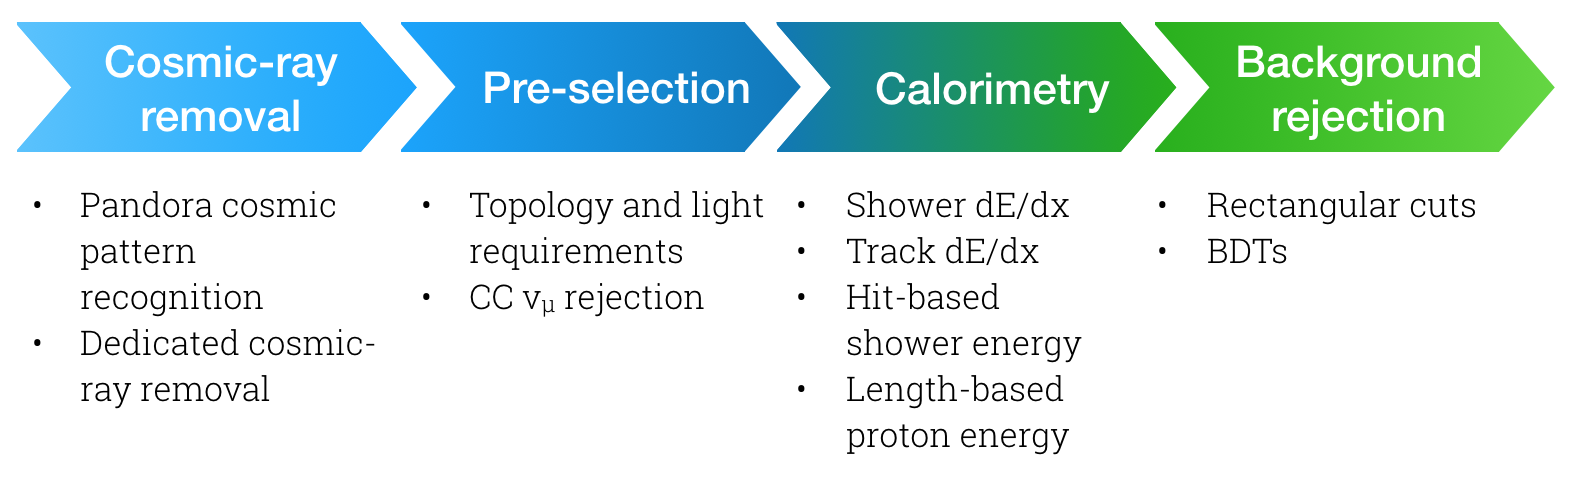
\includegraphics[width=0.9\linewidth]{figures/selection.png}
  \caption{Schematics of the $\nu_e$ CC0$\pi$-Np event selection stages.}
  \label{fig:selection}
\end{figure}

\subsection{Cosmic-ray rejection}\label{sec:cosmicremoval}
The hits in the TPC, reconstructed with the procedure described in Section \ref{sec:eventreco}, are passed to the Pandora framework for pattern recognition. The framework can run in two different modes: one optimised for the reconstruction of cosmic rays and delta rays (\emph{cosmic mode}), and one optimised for the reconstruction of neutrino interactions (\emph{neutrino mode}).

In order to reject the cosmogenic background, Pandora is first run in cosmic mode over all the reconstructed hits. This reconstruction is track-oriented, and the delta rays are reconstructed as showers and considered as daughters of the closest cosmic muon. The starting point of the reconstructed tracks in this mode is assumed to be the highest $y$ coordinate \cite{Acciarri:2017hat}.
These reconstructed high-level objects are fed to a series of cosmic-ray tagging algorithms, which we will briefly describe below.
\begin{description}
\item[Geometry and timing algorithm.] This algorithm checks if the reconstructed hits have a time compatible with the drift-time window. If a track or a shower has more than four hits outside the allowed drift-time window, then they are tagged as cosmic rays. Then, the algorithm loops over all the reconstructed objects and tag them if they have a trajectory that enters and exits the TPC borders, within a fiducial volume. The fiducial volume has been chosen by taking into account the magnitude of the space charge effect (Section \ref{sec:ionisation}).
\item[Optical algorithm.]{This algorithm takes into account the information provided by the optical system to reject cosmic rays interacting during the readout window. The algorithm first requires the presence of a reconstructed flash during the beam-spill window of 1.6~\si{\micro}s. Then, for each reconstructed particle a \emph{flash hypothesis} is built, meaning that we create a distribution of the light collected by each PMT compatible with the charge distribution of the reconstructed particle. The reconstructed particle is tagged as a cosmic ray if its hypothetical flash satisfies two requirements:
\begin{enumerate}
    \item at least one PMT sees an amount of PE $3\sigma$ larger than the reconstructed one.
    \item the hypothetical $z$ coordinate of the flash is not compatible with the $z$ coordinate of the reconstructed flash.
\end{enumerate}}

\item[Anode-Cathode Piercing Tracks algorithm.] The coordinate along the drift direction (which in MicroBooNE is the $x$ coordinate) can be reconstructed in a LArTPC only by knowing also the time $t$ when the particle interacted in the detector. The $x$ coordinate is then given by:
\begin{equation}
    x = v_{\mathrm{drift}}t,
\end{equation}
where $v_{\mathrm{drift}}$ is the drift velocity. In the case of a neutrino interaction, the time $t$ correspond to the beam trigger (plus a definite interval), while for a cosmic ray cannot be known without an external cosmic-ray tagger.
However, for the subset of cosmic rays piercing the cathode (or the anode) we will have:
\begin{align}
    t_{S(E)} - t_F \sim t_{C(A)},\label{eq:acpt}
\end{align}
where $t_S$ ($t_E$) is the time of the track start point (end point), $t_F$ is the time of the flash corresponding to the track, and $t_C$ ($t_A$) is the time corresponding to the position of the cathode (anode). Thus, for each track we loop over all reconstructed flash and we consider the track of cosmic origin if there is a flash which satisfies condition \eqref{eq:acpt}.

\item[Stopping-muon algorithms.] Cosmic muons which enter the TPC and stop in the liquid argon can be reconstructed as a track (the cosmic muon) and a shower (the Michel electron). Figure \ref{fig:michel_evd} shows a data event display of the collection plane with a muon stopping and decaying, producing a Michel electron. 

\begin{figure}[htbp]
\centering
  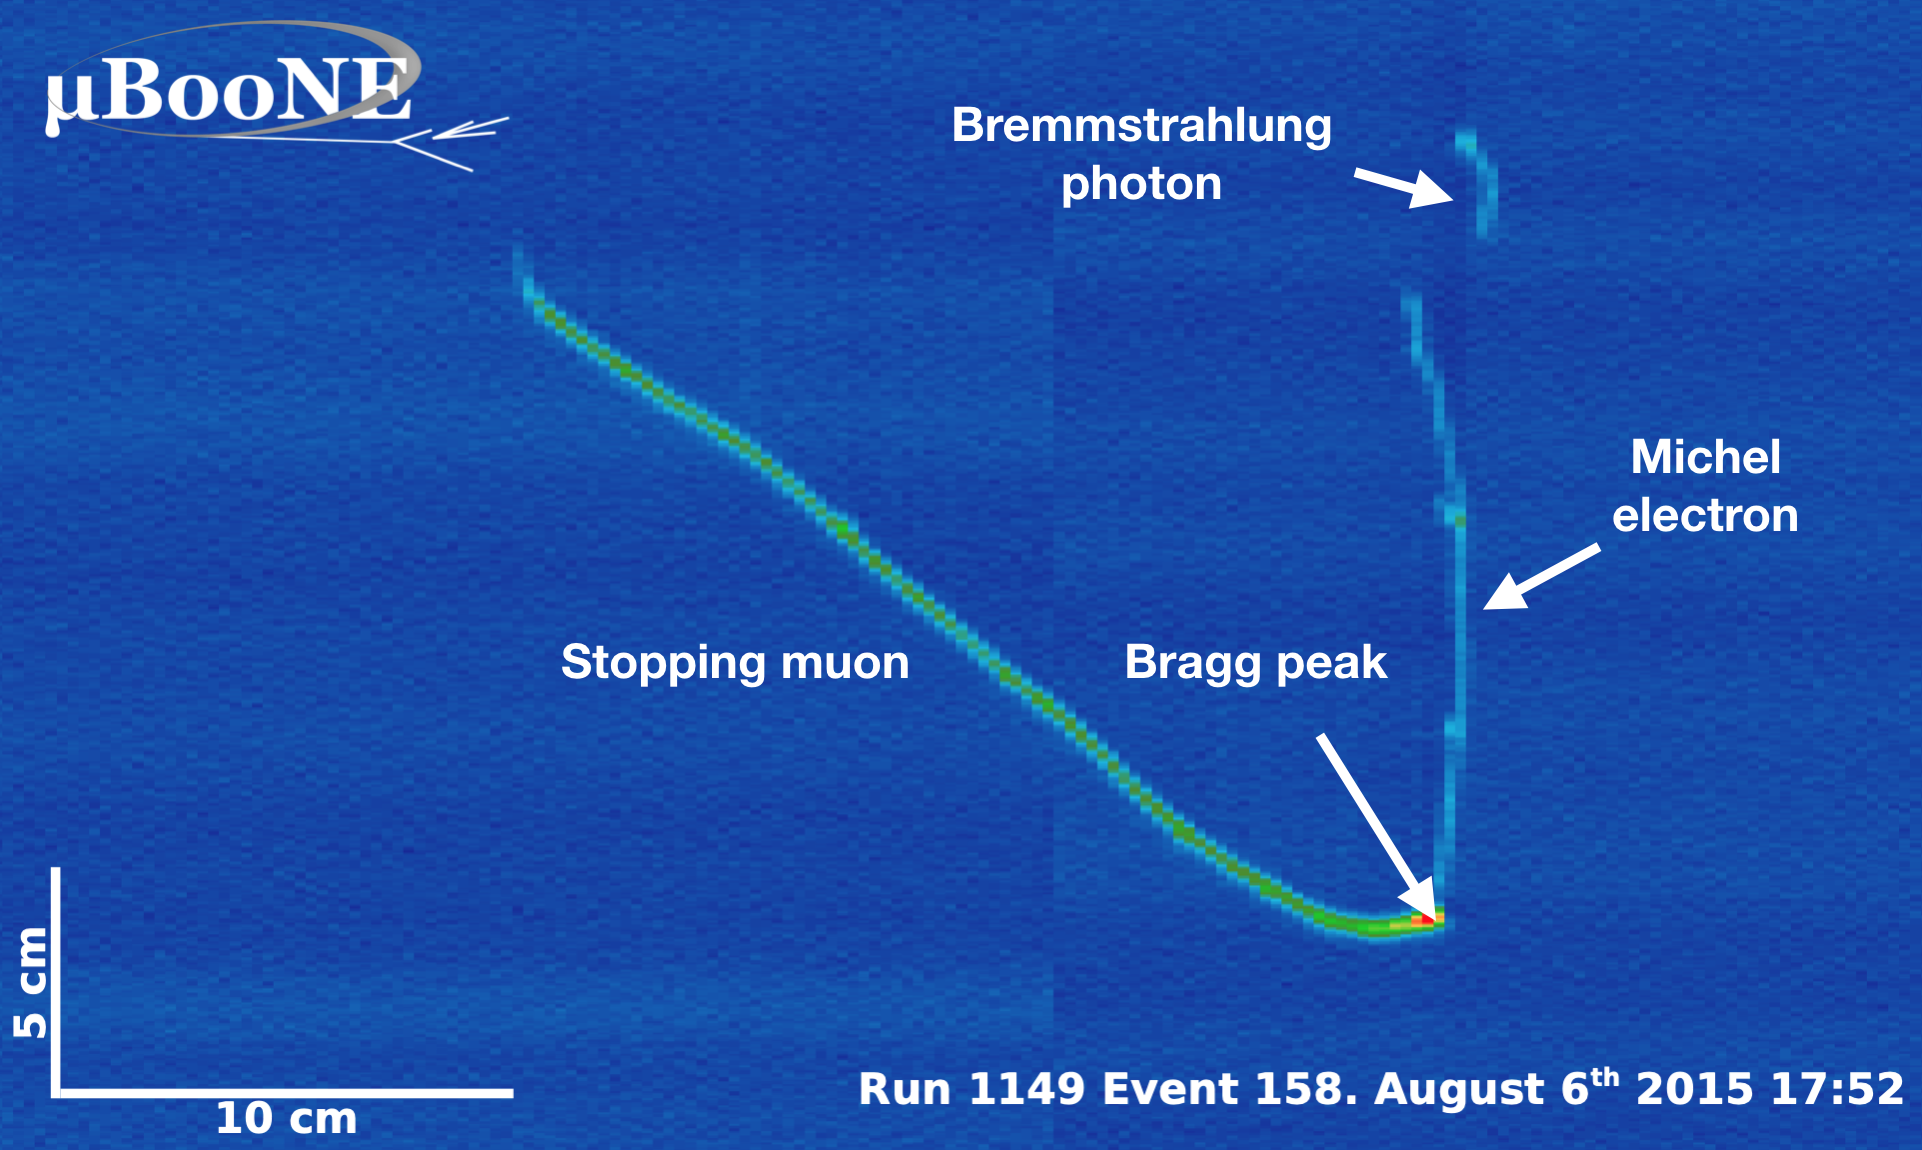
\includegraphics[width=0.75\linewidth]{figures/michel_evd.png}
  \caption{Event display of the collection plane with a muon stopping and decaying, producing a Michel electron.}
  \label{fig:michel_evd}
\end{figure}

This topology is similar to the one of an electron neutrino interaction. For this reason, stopping muons represent an important background for our analysis. 
They are tagged in two ways:
\begin{itemize}
    \item a series of pattern recognition and calorimetric algorithm try to identify the correct direction of the cosmic muon track (by measuring its energy loss profile) and to verify the presence of a \emph{kink} in the trajectory, caused by the presence of the Michel electron.
    \item the multiple Coulomb scattering (MCS) angle of a stopping muon will increase as its momentum decrease, while for through-going muons it is essentially constant \cite{Abratenko:2017nki}. By fitting the track profile with the MCS hypothesis in both direction (up-going and down-going), it is possible to verify if the cosmic muon is stopping in the detector. 
\end{itemize}

\end{description}

The hits associated with the tagged reconstructed objects (and to their daughters) are removed from the collection of reconstructed hits. The remaining hits are then fed to Pandora in \emph{neutrino mode}, which provides one or more neutrino interaction candidate per event. 

\subsection{Optical selection}\label{sec:optical_pre_cuts}
The optical selection serves two purposes: (1) it ensures that the optical flash which triggered the detector readout is compatible with the neutrino candidates from the Pandora neutrino mode, and (2) it provides a way to discriminate between multiple Pandora neutrino candidate objects (most of which are of cosmic origin) by selecting the one most compatible with the flash in the optical detection system in time with the beam-gate window.

The optical selection algorithm consists of three major stages:
\begin{enumerate}
\item cuts applied to optical properties of the reconstructed flash object (number of photoelectrons a TPC charge/PMT photoelectrons ratio);
\item cuts on the compatibility of the reconstructed flash with the Pandora neutrino candidate (position of the flash compared with the position of the centre of the collected charge);
\item the Pandora neutrino candidate which is most compatible with the flash is picked using a likelihood method.
\end{enumerate}

The effects of the optical selection have been studied in detail using the $\nu_{e}$~CC0$\pi$-Np + cosmic Monte Carlo sample, here our \emph{signal}, and the data beam-off sample, the \emph{background}.

We first require a reconstructed flash in the optical system within the beam spill window of \SI{1.6}{\micro\s}. This requirement selects the 99.6\% of the signal events ($\nu_{e}$ CC0$\pi$-Np) and 18.5\% of the background events (data beam-off). 
The reconstructed flash must also correspond to at least 50 PE recorded by the optical system. This is a very conservative requirement and keeps 99.95\% of the signal and 95.2\% of the background (Figure \ref{fig:pe_cut}).

\begin{figure}[htbp]
\centering
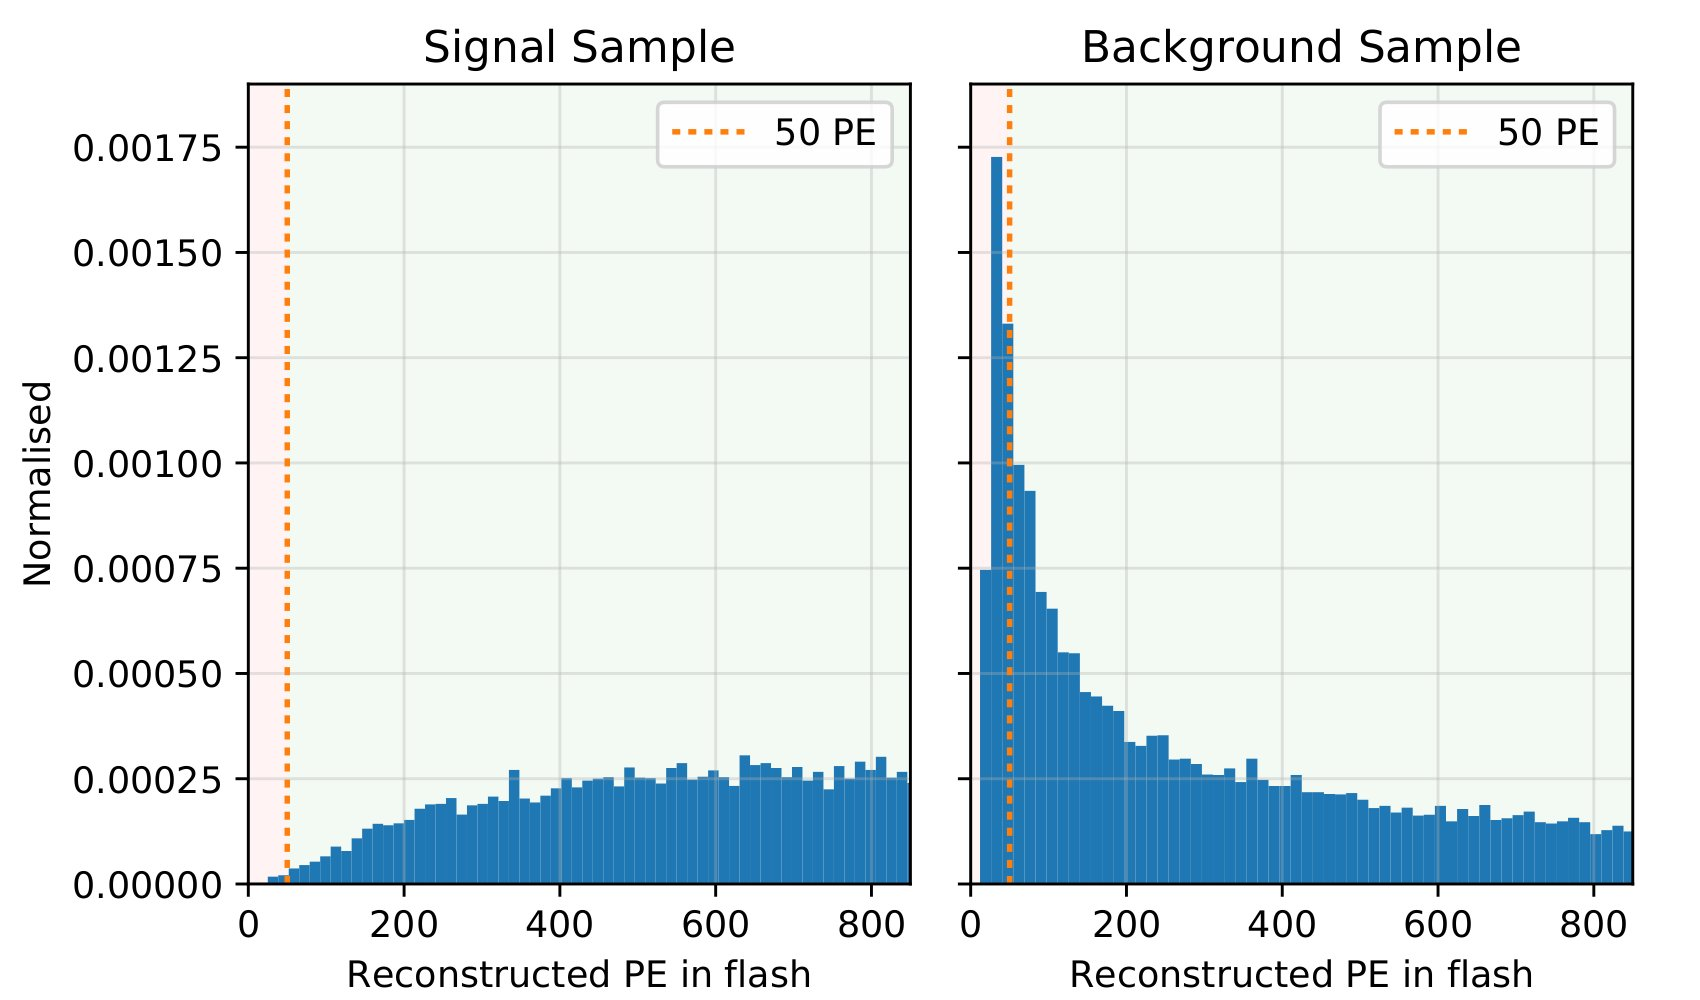
\includegraphics[width=0.85\textwidth]{figures/pe_cut.jpg} 
\caption{Reconstructed PE distribution for signal (left) and background (right) events.} 
\label{fig:pe_cut}
\end{figure}

These two cuts ensure that the event has a properly reconstructed flash. A flash object has a time and a PE count for each of the 32 PMTs. From this information, two coordinates $z\pm \sigma_z$ and $y\pm \sigma_y$ are calculated, where the positive $z$ axis corresponds to the beam direction and $y$ coordinate corresponds to the detector height. These two values can be compared with the centre of the deposited charge of the reconstructed neutrino candidate in the TPC. This comparison has the implicit assumption that the light will be emitted in the same relative fraction as the charge deposited by the particles in the final state. This is not completely correct since the amount of scintillation light produced per deposited energy unit depends on the particle. Nevertheless, the coarse resolution given by the PMT grid allows to use this approximation.

A cut of \SI{105}{\cm} is placed on the difference between the reconstructed flash position and the centre of the deposited charge on the $z$ axis. This cut keeps at least one neutrino candidate in 98.1\% of the signal events, and it removes all neutrino candidates in 20\% of the background events (Figure \ref{fig:z_cut}). 
Similar cuts are placed taking into account the width of the flash and its position on the $y$ axis. 

\begin{figure}[htbp]
\centering
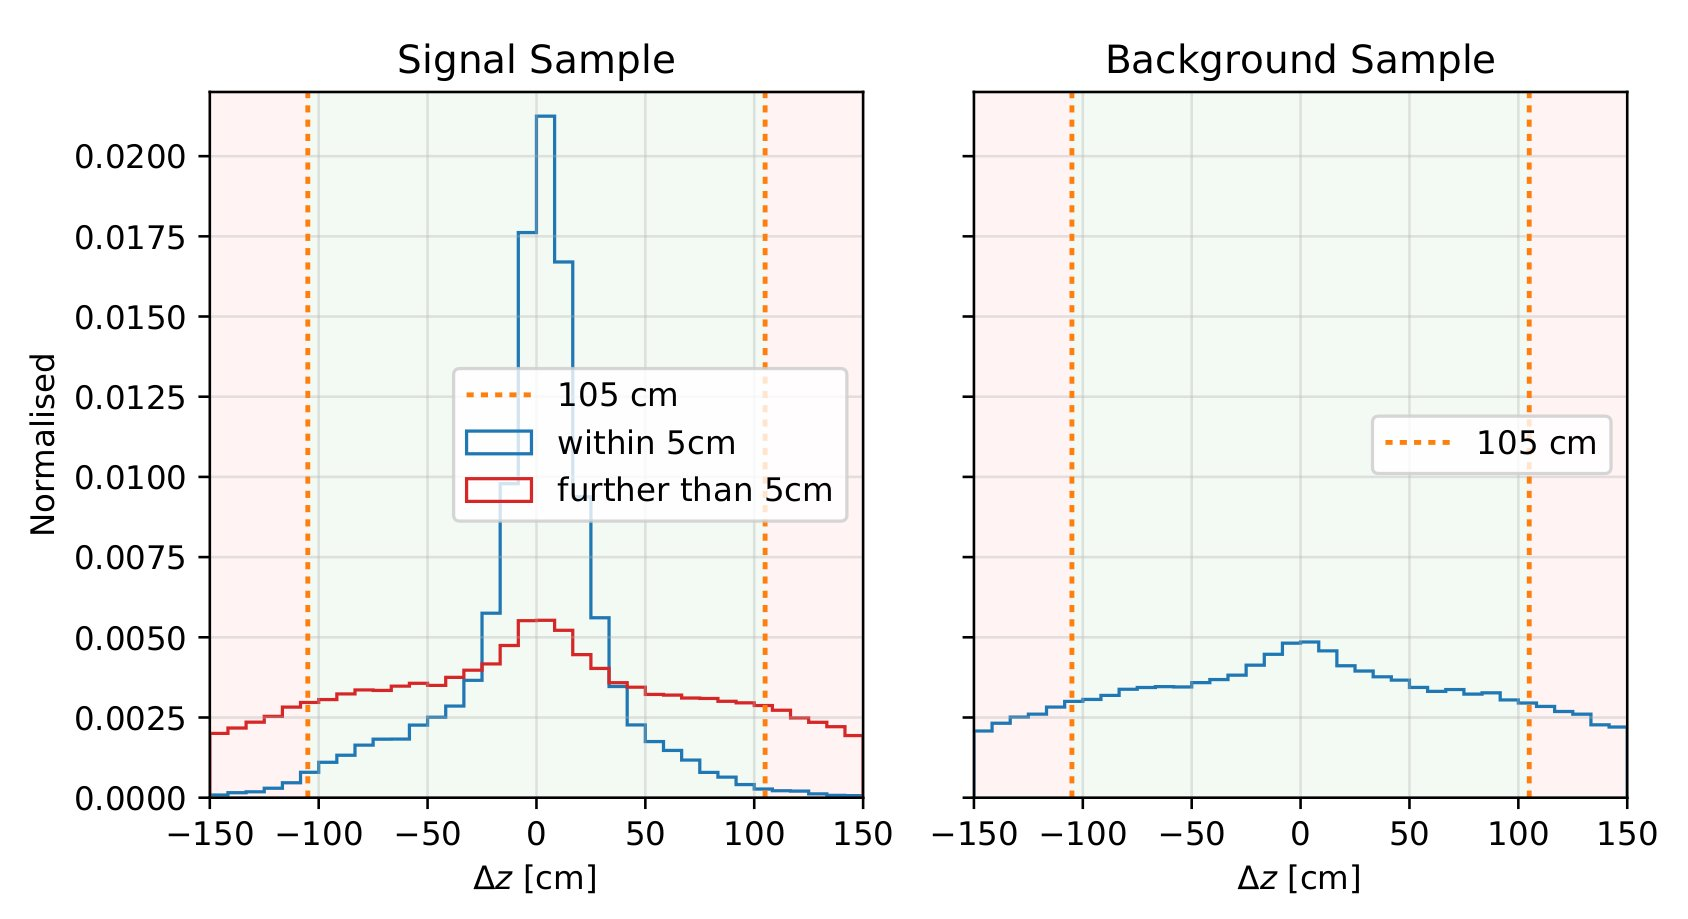
\includegraphics[width=0.85\textwidth]{figures/z_cut.jpg} 
\caption{Distribution of the distance between the reconstructed flash position and the centre of the deposited charge on the $z$ axis for signal (left) and background (right). The \emph{within 5 cm} and \emph{further than 5 cm} categories refers to the distance between the reconstructed neutrino vertex and the true neutrino vertex.} 
\label{fig:z_cut}
\end{figure}

The last rectangular cut exploits the fact that several neutrino candidates reconstructed by Pandora originate from remnants of cosmic activity which were not tagged by the cosmic-removal algorithms. Those neutrino candidates often consist in a small amount of fragmented charge, incompatible with the brightness of the flash. Placing a very conservative cut at 3.0 on the ratio between the charge in the collection plane associated to the neutrino candidate and the number of PEs reduces the signal events with a properly reconstructed flash by 1.7\%, while removing all neutrino candidates in 15.4\% of the background events (Figure \ref{fig:light_ratio}).

\begin{figure}[htbp]
\centering
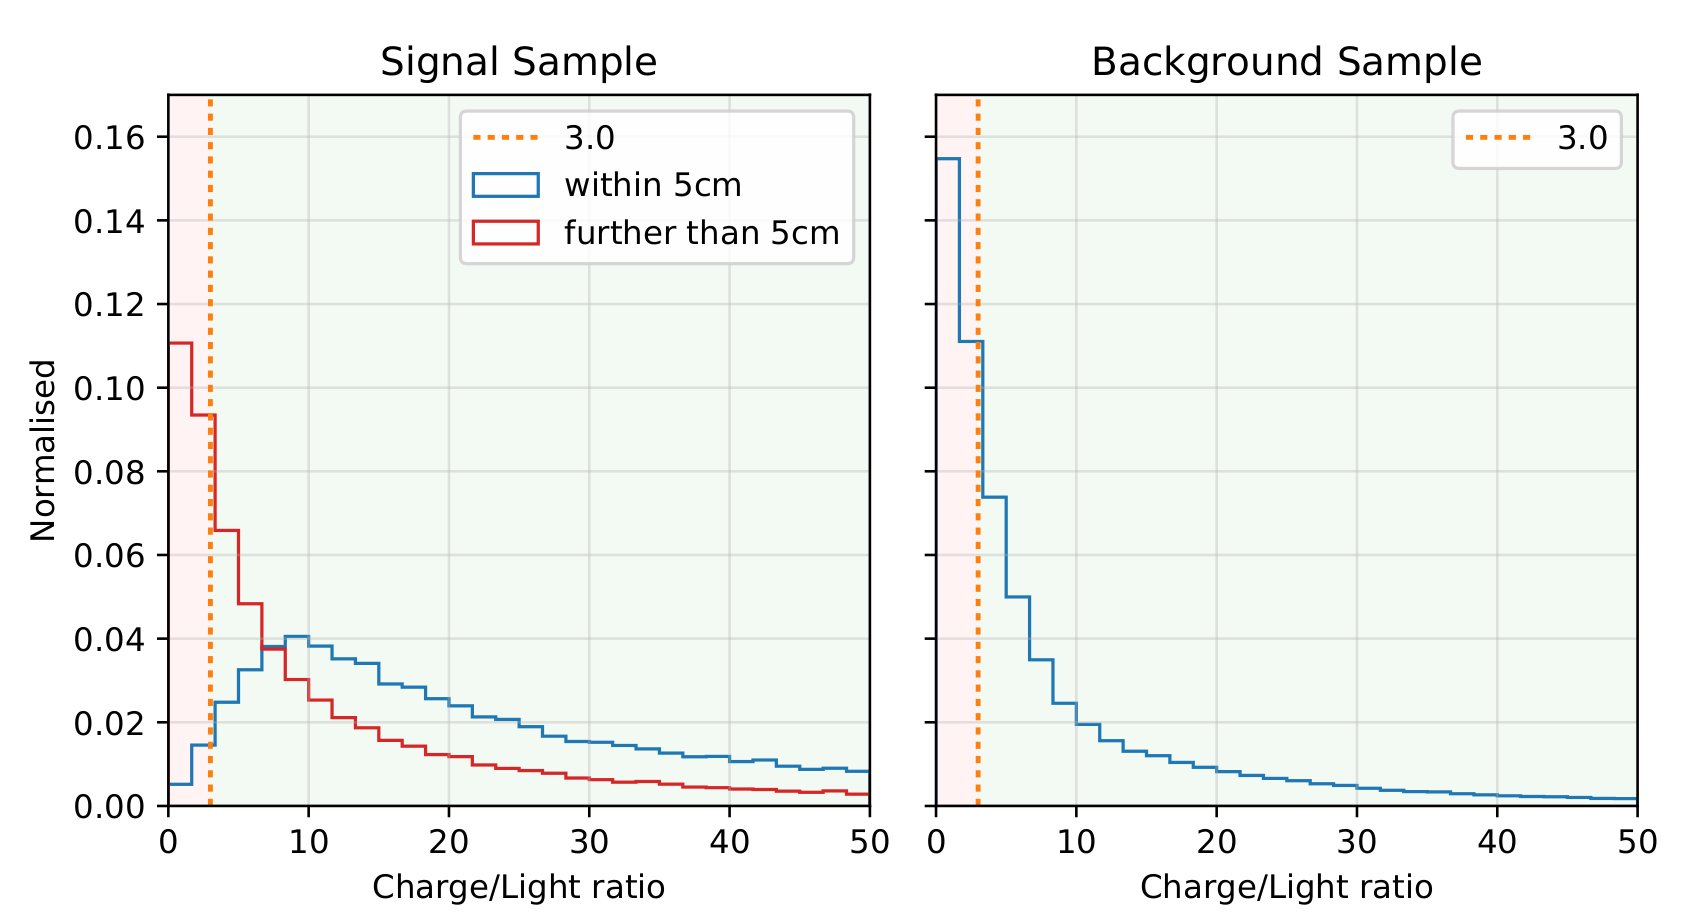
\includegraphics[width=0.85\textwidth]{figures/light_ratio.jpg} 
\caption{Distribution of the ratio between the charge in the collection plane associated to the neutrino candidate (in ADC counts) and the number of PEs collected by the PMTs. The \emph{within 5 cm} and \emph{further than 5 cm} categories refers to the distance between the reconstructed neutrino vertex and the true neutrino vertex.} 
\label{fig:light_ratio}
\end{figure}

After these rectangular cuts it is still possible to have more than one reconstructed neutrino candidate in the event. A flash-matching procedure allows to choose the one that best matches the collected light:
\begin{enumerate}
\item a flash hypothesis is made for each candidate, using the information from the TPC;
\item for every neutrino candidate, a spatial distribution of deposited charge is measured;
\item the spatial distribution of the deposited charge is translated into an estimation of the emitted scintillation light. These scintillation photons are then propagated towards the PMTs to construct a flash hypothesis using only TPC information;
\item the flash-matching algorithm compares the reconstructed flash object as seen by the PMTs with the hypothetical flash for every reconstructed neutrino candidate and picks the best-matching candidate. This selection is achieved through a binned likelihood of the PMT spectrum.
\end{enumerate}


An example of this procedure for a Monte Carlo generated $\nu_e$ event with 4 neutrino candidates is given in Figure~\ref{fig:flashmatch}.

\begin{figure}[htbp]
\centering
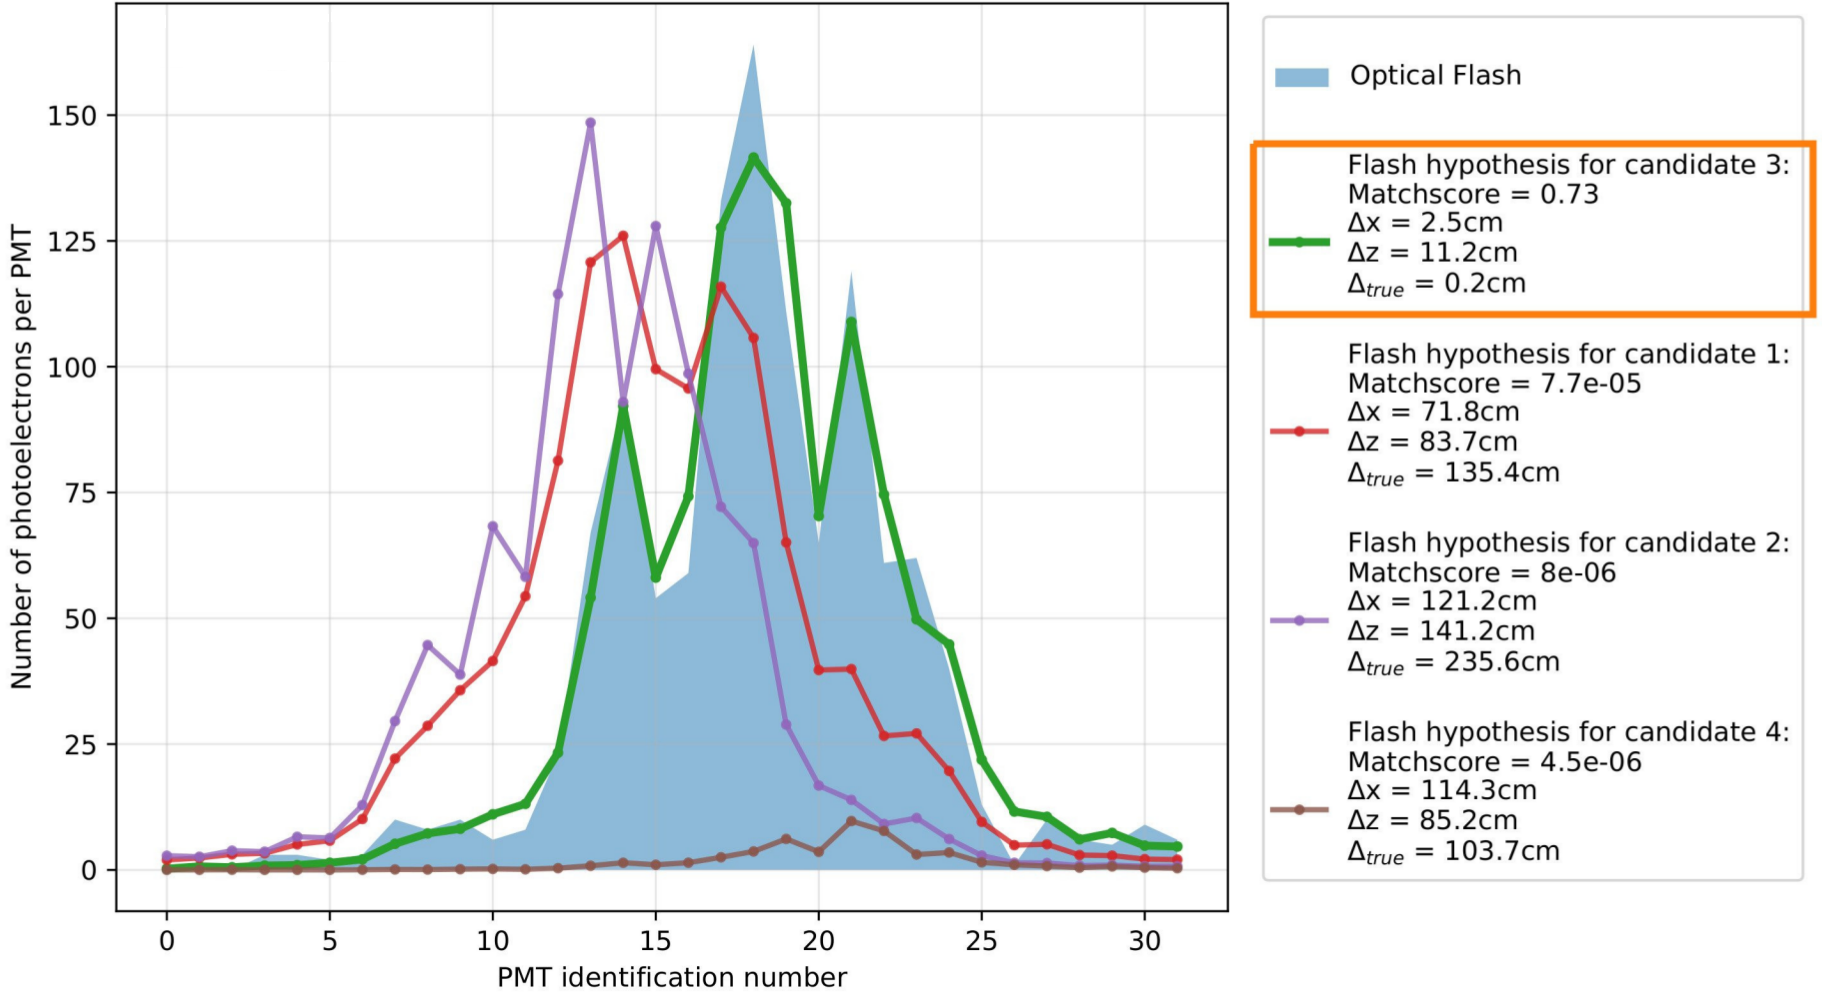
\includegraphics[width=0.85\textwidth]{figures/flashmatch.png} 
\caption{An example of flash-matching. The event has 4 neutrino candidates and we make a flash hypothesis for each one. A minimum binned likelihood is calculated, varying the $x$ position of the interaction. The match score is the inverse of the likelihood. The candidate with the highest match score is chosen as neutrino interaction candidate.} 
\label{fig:flashmatch}
\end{figure}

\subsection{Topological pre-selection} \label{sec:topological_pre_selection}
A perfect reconstruction of a $\nu_{e}$ CC0$\pi$-Np event in a LArTPC will produce as many reconstructed tracks as the number of protons above the detection threshold in the final state and a single reconstructed shower (the electron), sharing a common vertex. However, mis-reconstruction and mis-classification issues can significantly lower the selection efficiency. The current status of the event reconstruction, which depends on the quality of the event (e.g. the number of hits \cite{Acciarri:2017hat}), affects the efficiency of selecting these events. For example, the presence of dead or unresponsive wires can affect the reconstruction by causing the splitting of an ionisation track or an electromagnetic shower into two distinct reconstructed objects. Also, the selection currently implemented relies on the classification of the reconstructed objects as track-like or shower-like, a separation that contains an inherent inefficiency associated, especially when the number of reconstructed hits is low.

In order to maximise our efficiency we currently require (1) \emph{at least} one track and \emph{at least} one shower sharing a common vertex, or (2) \emph{at least} two showers sharing a common vertex, to account for proton mis-classification as a shower-like object. For these cases we measure the $\chi^2$ score of the $dE/dx$ vs. residual range profile of the reconstructed objects in the proton hypothesis, as described in Section \ref{sec:proton_id}. The object with the lowest $\chi^2$ score is considered as a track, while the remaining ones are considered as showers.

\subsection{Minimum quality requirements}\label{sec:precuts}
A minimal set of cuts is applied to the selected events, in order to ensure that they are well reconstructed.
First, to avoid border effects, the reconstructed neutrino vertex, the start point of the reconstructed showers and the start and end points of the reconstructed tracks are required to lie within a fiducial volume. Our fiducial volume cut is 10~cm from each side on the $x$ axis, 15~cm from each side on the $y$ axis, and 10~cm (40~cm) from the upstream (downstream) side on the $z$ axis. 
Since electromagnetic showers develop mainly in the forward direction with respect to the beam, the asymmetric cut on the $z$ axis (which corresponds to the beam direction) helps reject non-fully contained events which begin too close to the downstream end of the TPC.
We also require, for each event, (1) at least 5 hits in the three planes associated to shower-like objects, (2) at least 5 hits in the three planes associated to track-like objects, and (3) at least one hit in every plane.


\subsection{Selection efficiency and purity}\label{sec:eff}
The selection efficiency of our algorithm is obtained by calculating the fraction of events selected in the $\nu_{e}$ CC$0\pi$-Np + cosmic Monte Carlo sample, where the true neutrino vertex, the start and end points of the protons, and the start point of the electron are fully contained in the fiducial volume.

In order to understand what energy thresholds are appropriate for reconstruction in the TPC, dedicated studies have been performed on proton tracks and electron showers, using the $\nu_{e}$ CC$0\pi$-Np + cosmic Monte Carlo sample. We have found that we have no efficiency for reconstructing and classifying protons {with a kinetic energy} below 40~MeV and electrons{, photons, and charged pions} {with a kinetic energy} below 30~MeV following these optical, topological, and minimum quality pre-selections. Therefore, these energy thresholds are applied to the simulations to allow a fair comparison with the reconstructed particles. 

Our overall $\nu_{e}$ CC$0\pi$-Np selection efficiency $\epsilon$ is defined as:
\begin{equation}
\epsilon = \frac{\mathrm{N.~of~selected~}\nu_{e}\mathrm{~CC0}\pi\mathrm{{\text -}Np~events}}{\mathrm{N.~of~generated~}\nu_{e}\mathrm{~CC0}\pi\mathrm{{\text -}Np~events}},
\end{equation}
where each selected event must pass the optical selection, satisfy the topology and minimum quality requirements, and not being vetoed by the independent CC $\nu_{\mu}$ selection module. Figure \ref{fig:thresholds} shows the selection efficiency as a function of the electron and the proton kinetic energies. 

\begin{figure}
\centering
  \begin{subfigure}{0.48\textwidth}
    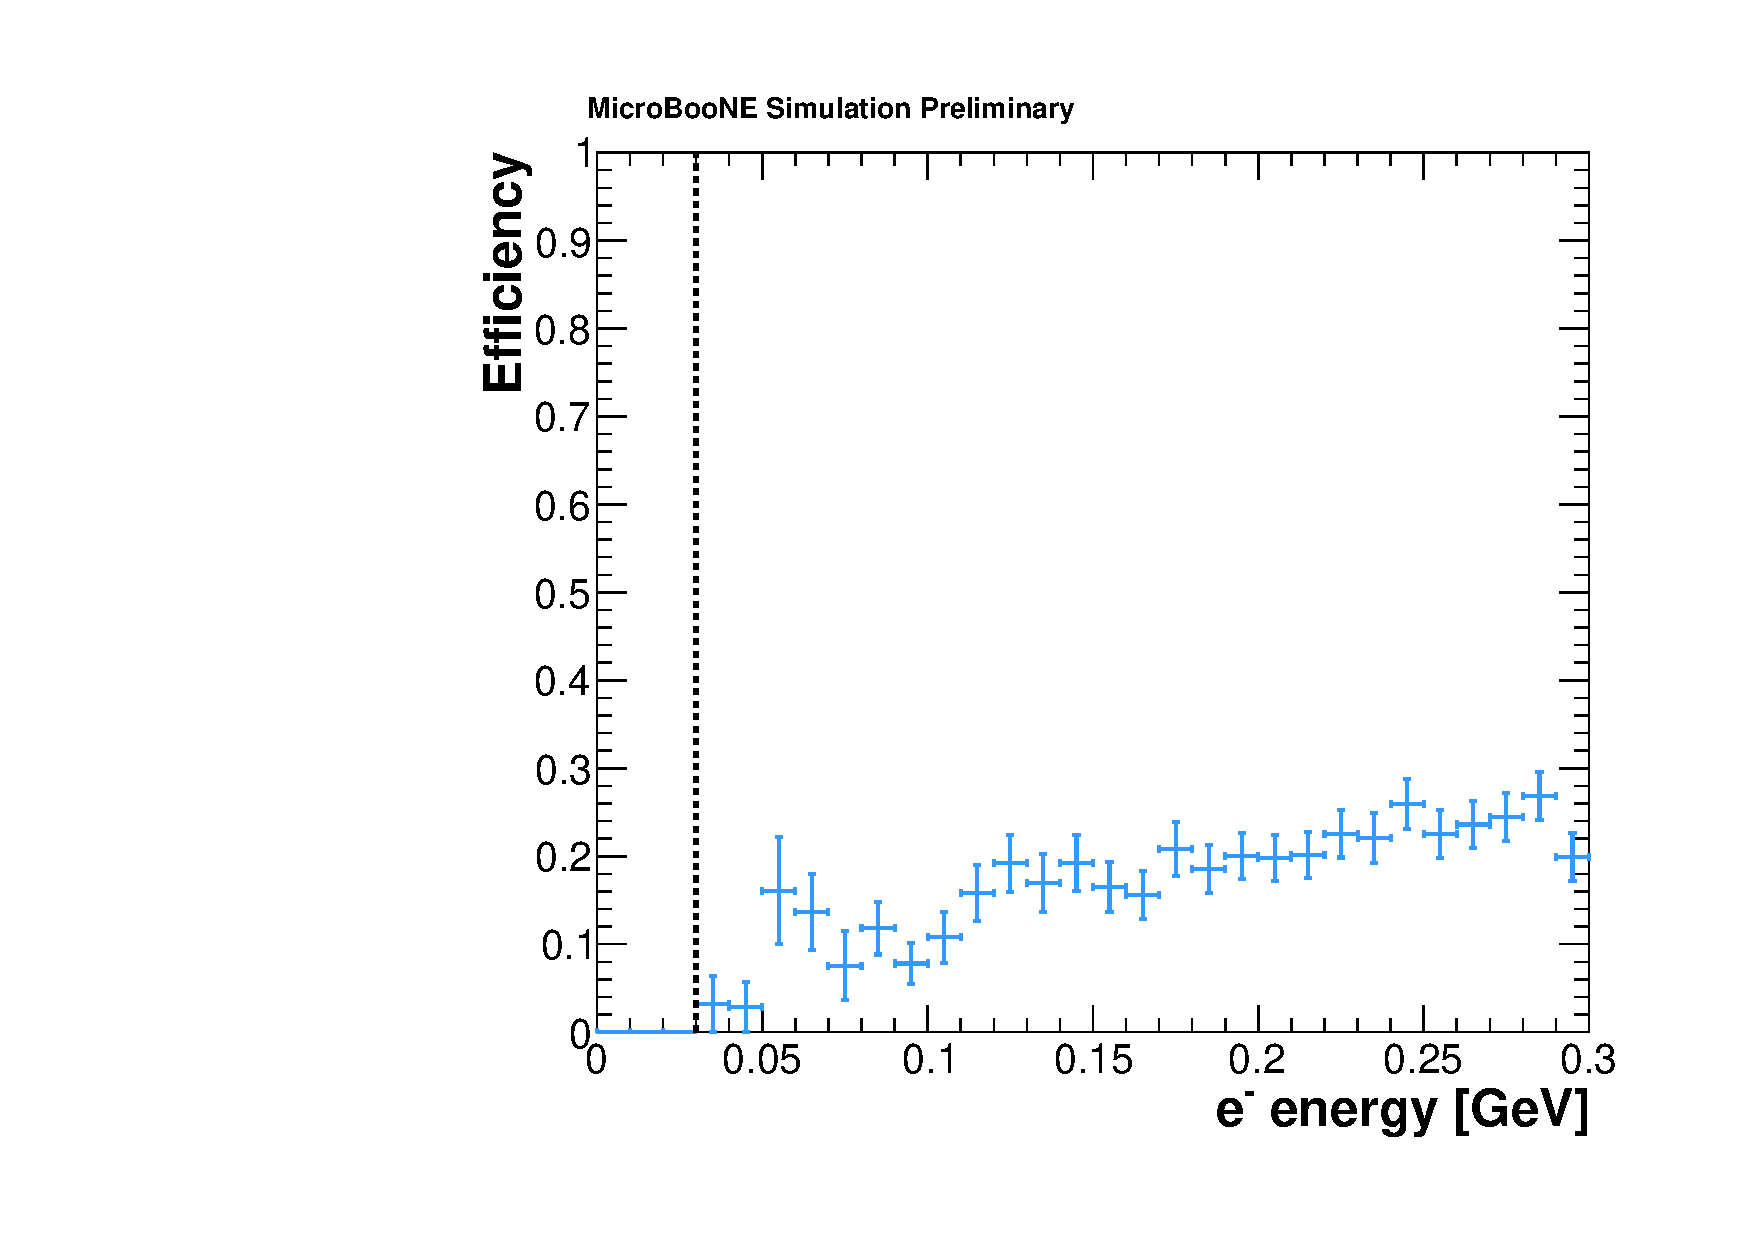
\includegraphics[width=\linewidth]{figures/e_efficiency.pdf}
    \caption{Electron efficiency.} 
  \end{subfigure}
    \begin{subfigure}{0.48\textwidth}
    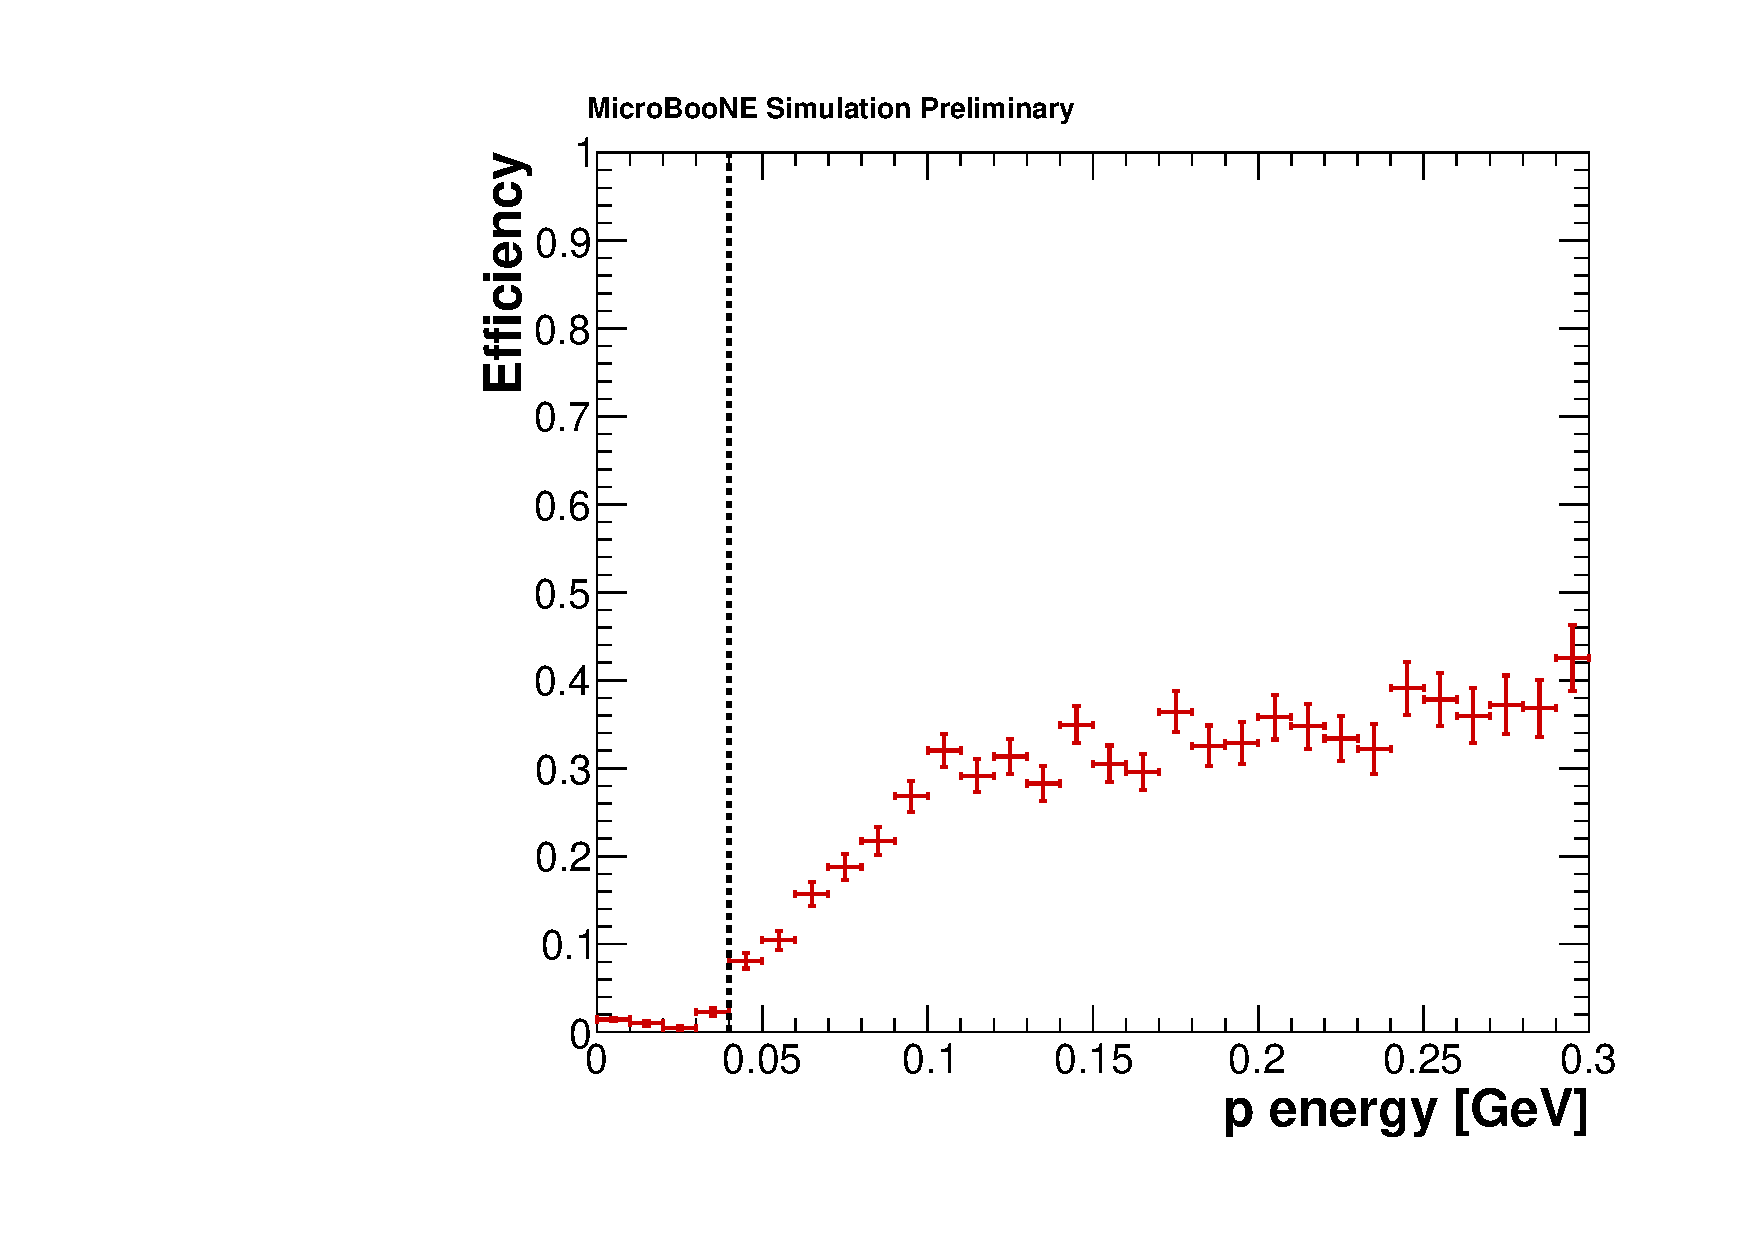
\includegraphics[width=\linewidth]{figures/p_efficiency.pdf}
    \caption{Proton efficiency.} 
  \end{subfigure}
  \caption{$\nu_{e}$ CC$0\pi$-Np selection efficiency as a function of the true electron (left) and proton (right) kinetic energy. The dashed lines correspond to the threshold applied at truth level.}
  \label{fig:thresholds}
\end{figure}


The true neutrino energy spectrum of the simulated $\nu_{e}$ CC$0\pi$-Np events in the 0-3~GeV range is shown in Figure \ref{fig:true_energy}.

\begin{figure}
\centering
  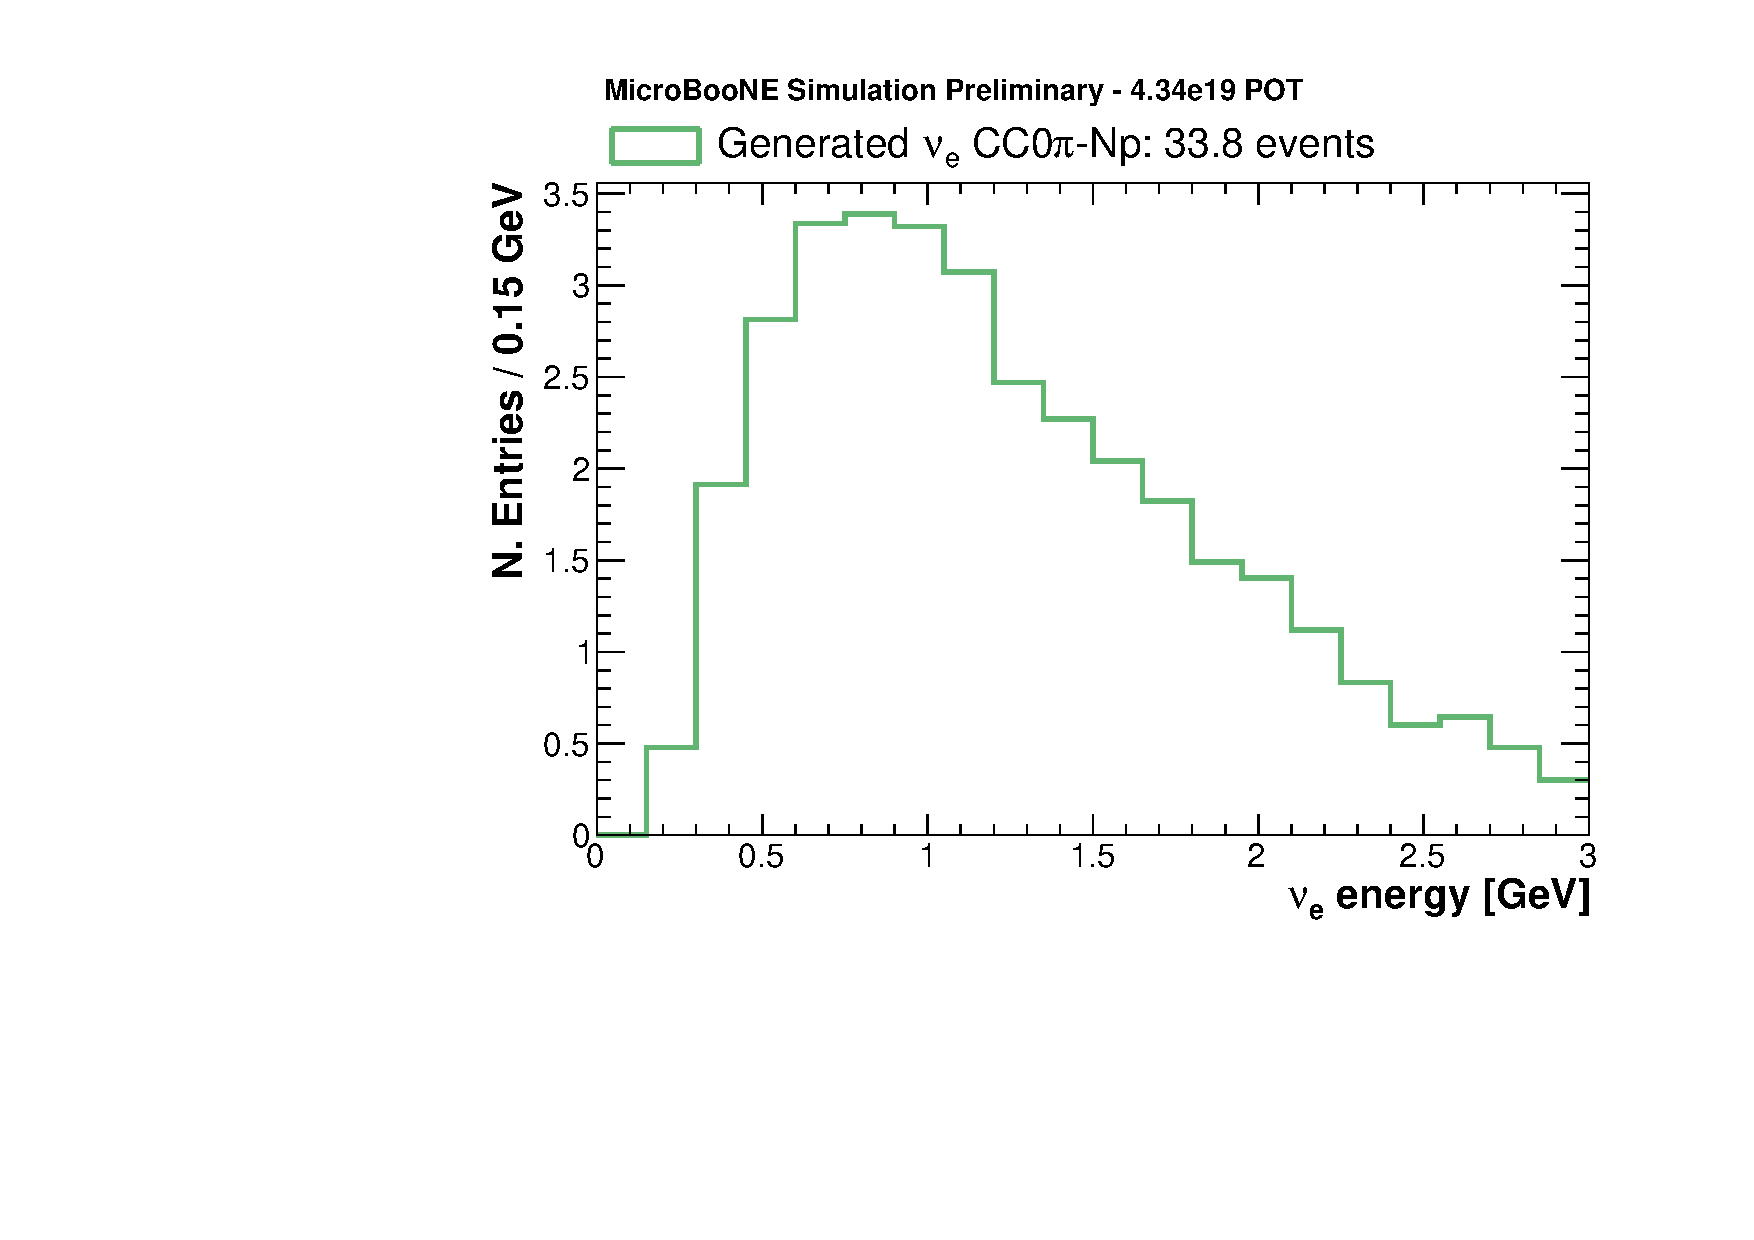
\includegraphics[width=0.8\linewidth]{figures/tot.pdf}
  \caption{$\nu_{e}$ CC$0\pi$-Np simulated true neutrino energy spectrum in the 0-3~GeV range. Each true proton (true electron) in the final state is required to have a kinetic energy larger than 40~MeV (30~MeV). The inner error bars represent the Monte Carlo statistical uncertainty, while the outer error bars are obtained summing in quadrature the statistical and the systematic uncertainties.}
  \label{fig:true_energy}
\end{figure}

Figure \ref{fig:effpurity} shows the efficiency as a function of the true neutrino energy.
%The energy reconstruction procedure is described in section \ref{sec:energyreco}.
The systematic uncertainties related to the cross-section and the neutrino beam flux, described in Section \ref{sec:systematics}, are also included. The inner error bars represent the Monte Carlo statistical uncertainty, while the outer error bars are obtained summing in quadrature the statistical and the systematic uncertainties. The statistical uncertainty $\delta\epsilon$ corresponds to the binomial error, since the application of a selection can be considered a binomial process \cite{Paterno:2004cb}:
\begin{equation}
    \delta\epsilon = \frac{1}{N}\sqrt{k(1-k/N)},
\end{equation}
where $k$ is the number of selected events and $N$ is the total number of events.

As expected, the efficiency increases with the neutrino energy, since high-energy events correspond in general to a larger number of hits in the TPC and the Pandora framework reconstruction performances increase with the number of reconstructed hits \cite{Acciarri:2017hat}. 

%A description of future improvements, which will allow us to increase the selection efficiency, is included in Section \ref{sec:future}.

% \todo{Add efficiency plots over a larger energy region for protons and electrons.}

\begin{figure}
\centering
%   \begin{subfigure}{0.48\textwidth}
    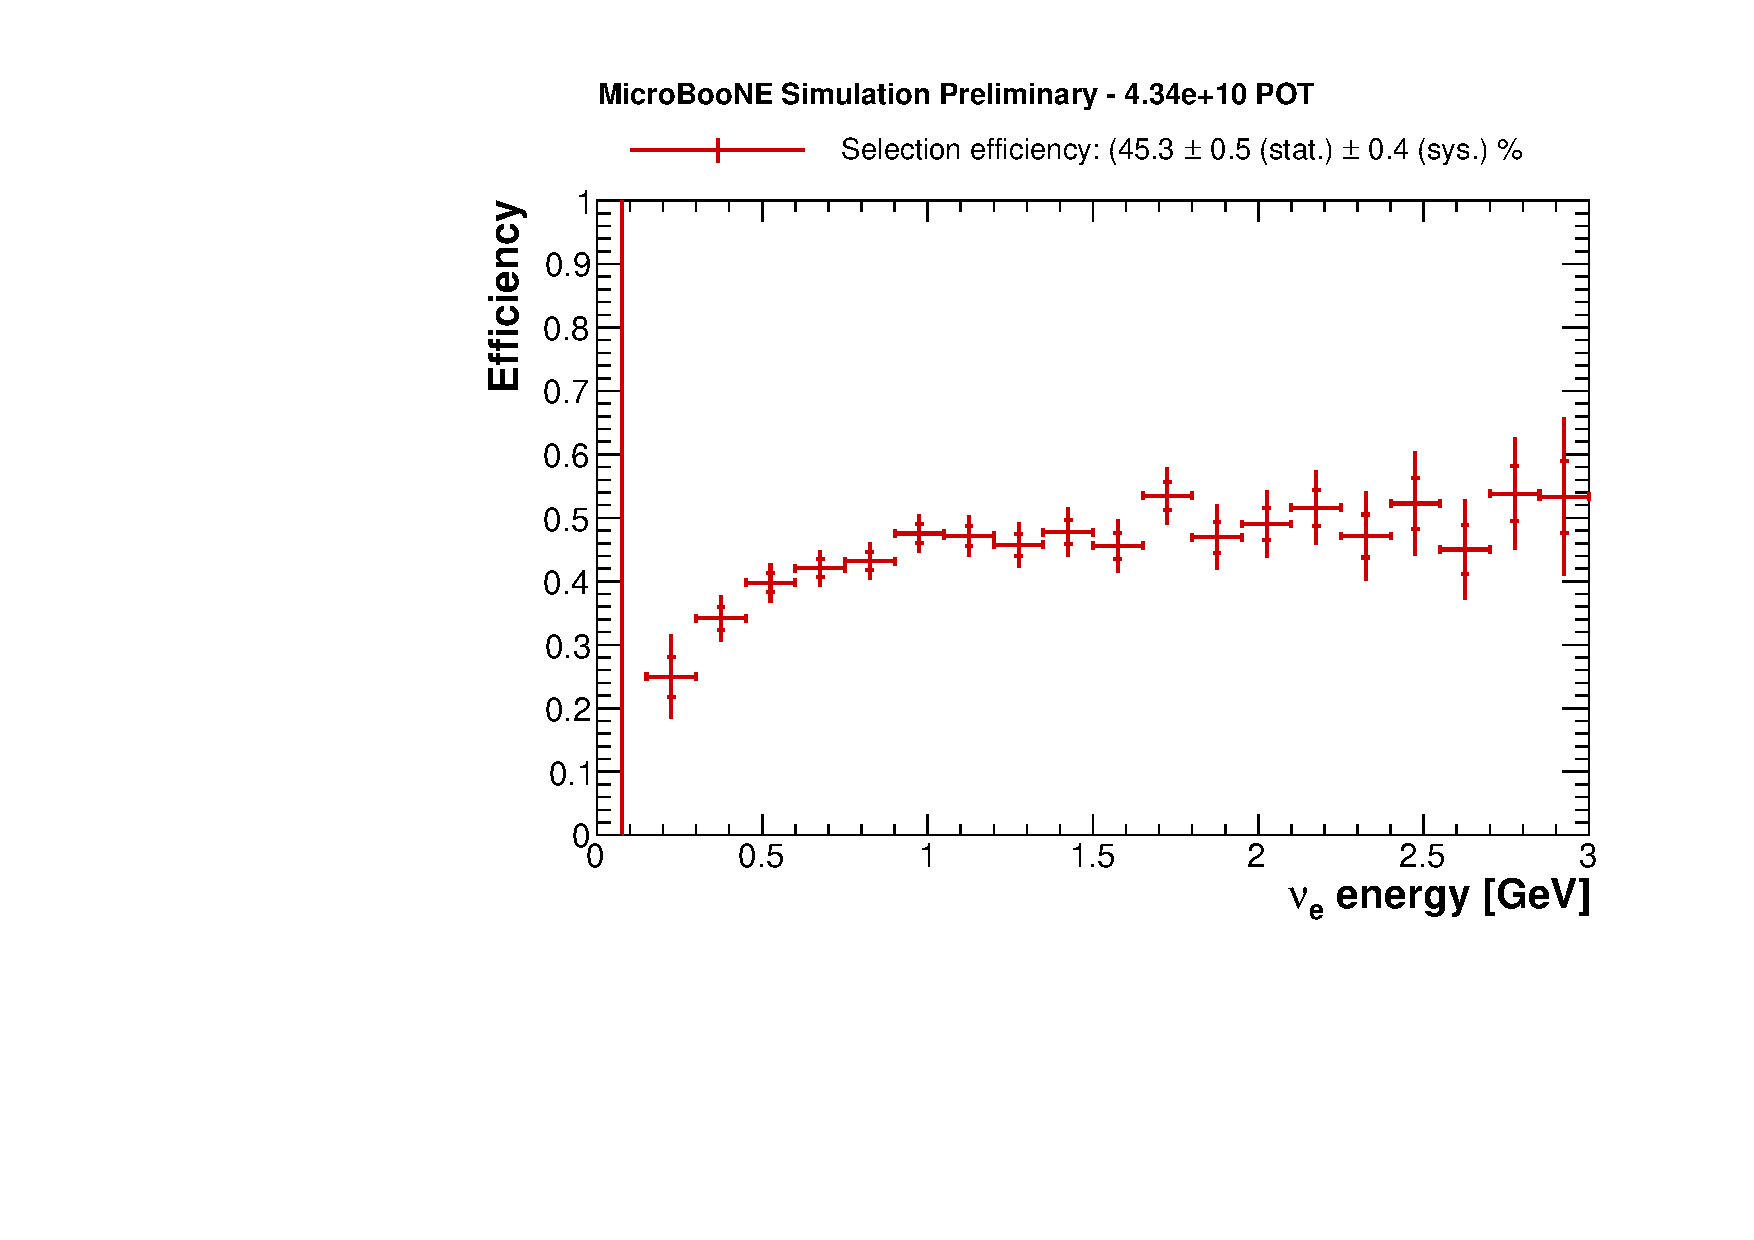
\includegraphics[width=0.8\linewidth]{figures/eff.pdf}
%     \caption{Efficiency.} 
%   \end{subfigure}
%     \begin{subfigure}{0.48\textwidth}
%     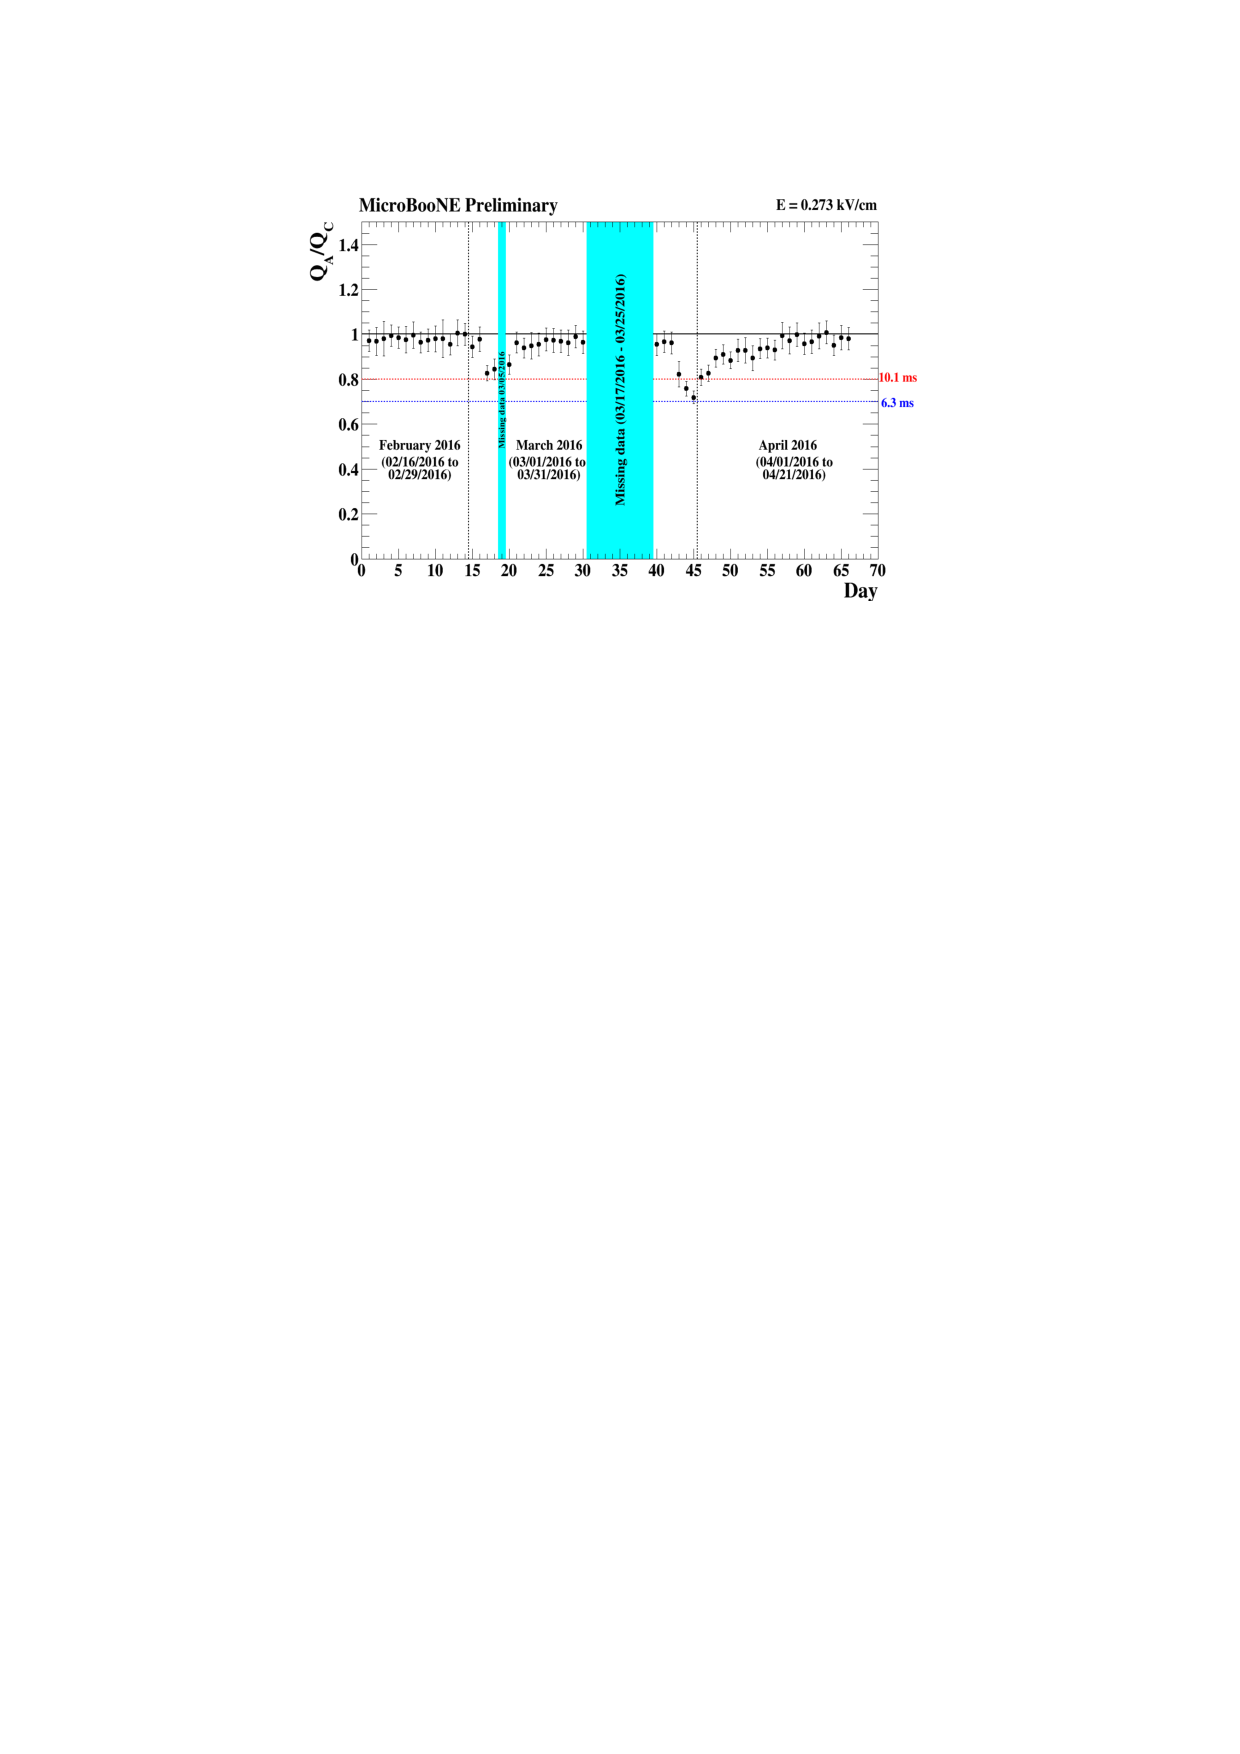
\includegraphics[width=\linewidth]{figures/purity.pdf}
%     \caption{Purity.} 
%   \end{subfigure}
  \caption{$\nu_{e}$ CC$0\pi$-Np selection efficiency as a function of the true $\nu_{e}$ energy. Each true proton (true electron) in the final state is required to have a kinetic energy larger than 40~MeV (30~MeV).}
  \label{fig:effpurity}
\end{figure}

\subsubsection{Inefficiencies breakdown}\label{sec:ineff}
Our current selection algorithm can fail for several reasons: in particular, we could have problems in the classification, such as an electron classified as a track-like object, or particles not reconstructed at all. We identified eight main causes for our selection inefficiency, whose contributions have been estimated with the same simulated sample described in Section \ref{sec:eff}:
\begin{description}

\item[Quality cuts (8.5\%).] {The selected neutrino candidate does not satisfy our minimum quality requirements, as described in Section \ref{sec:precuts}.}
\item[CC $\nu_{\mu}$ selected (4.3\%).]  {The event is tagged as a CC $\nu_{\mu}$ candidate by an independent selection module, described in \cite{ubxsec}}. 
\item[Not contained (10.1\%).] {One of the reconstructed tracks or the starting point of one of the reconstructed showers is not contained in the fiducial volume. As expected, this fraction increases with the neutrino energy}.
\item[Cosmic selected (7.9\%).] {The selected neutrino candidate has one or more reconstructed objects of cosmic origin}.
\item[1 shower (3.5\%).] {The selected neutrino candidate has only one associated reconstructed shower and no other object}. 
\item[No showers (13.7\%).]  {The selected neutrino candidate has only reconstructed track(s) associated. This is the largest contribution to the inefficiency, especially at low energies, since low-energy electrons are very challenging to reconstruct and classify as showers.}
\item[No flash (5.7\%).]  {The flash collected by the optical system does not satisfy our requirements, described in Section \ref{sec:optical_pre_cuts}}.
\item[No data products (0.7\%).] {The event does not have any neutrino candidate}.
\end{description}

Figure \ref{fig:ineff} shows a stacked histogram of the true neutrino energy for the $\nu_e$~CC0$\pi$-Np generated events, divided into the categories described above. The events without a reconstructed shower are the dominant inefficiency at low energy. The fraction of events where at least one reconstructed object is not contained in the detector (\emph{not contained} in the legend) increases with the energy. This is expected, since the probability to have large electromagnetic showers split in two or more object increases, and these objects can have a vertex reconstructed outside the fiducial volume. The \emph{passed} category (filled grey histogram) corresponds to the efficiency plot shown in Figure \ref{fig:effpurity}.

\begin{figure}
\centering
  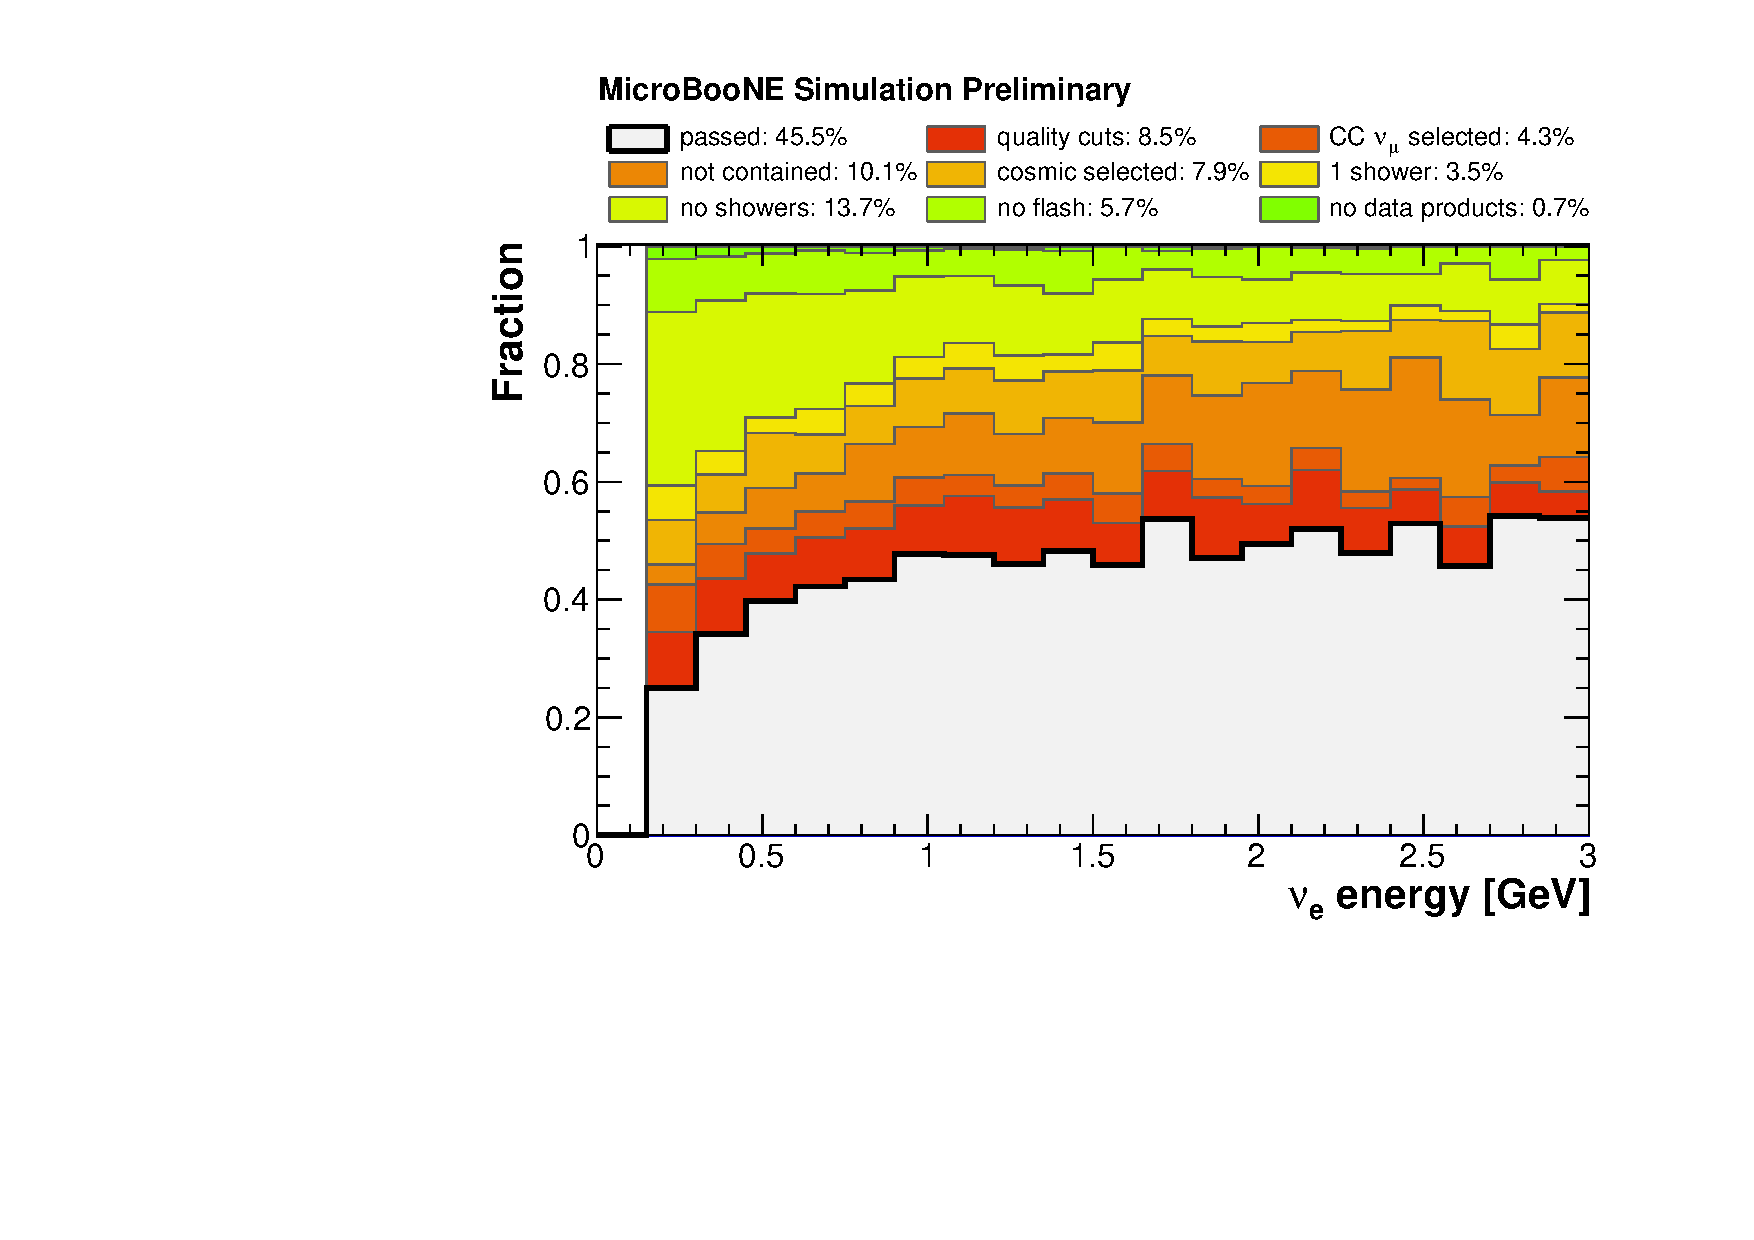
\includegraphics[width=0.8\linewidth]{figures/ineff_ene.pdf}
  \caption{Stacked histogram of generated events as a function of the true neutrino energy, categorised into correctly identified signal events {(\emph{passed})} and different reconstruction or identification failure modes.}
  \label{fig:ineff}
\end{figure}

The selection outcomes as a function of the lepton true angular variables $\theta$ and $\phi$ are shown in Figure \ref{fig:ineff_angles}. The efficiency is mostly constant as a function of the azimuthal angle $\phi$, while the fraction of events without reconstructed showers increases as a function of the $\theta$ angle. This is because backwards-going electrons are more difficult to reconstruct, since they are often low-energetic and pattern recognition groups the electron hits together with the forward-going proton track.

\begin{figure}
\centering
  \begin{subfigure}{0.48\textwidth}
    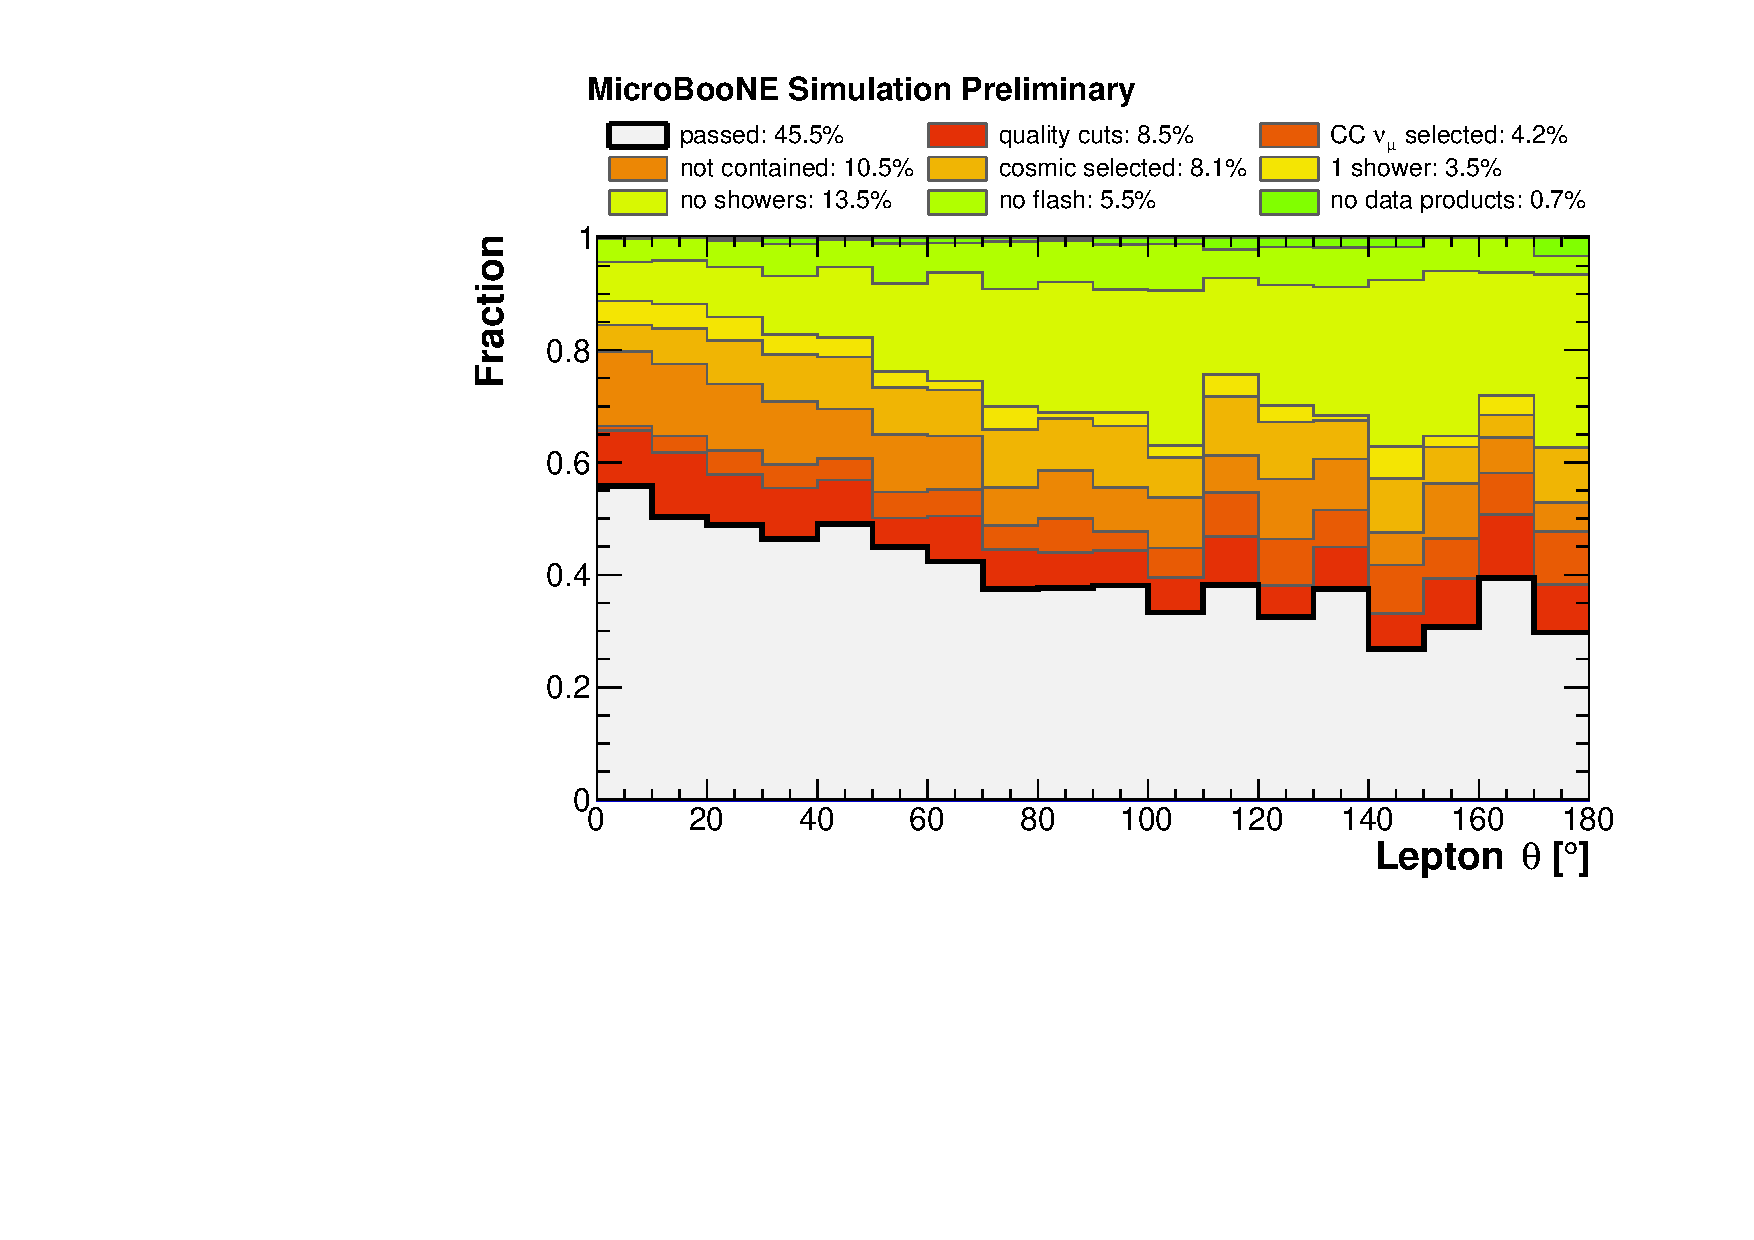
\includegraphics[width=\linewidth]{figures/ineff_theta.pdf}
    \caption{$\theta$ efficiency} 
  \end{subfigure}
    \begin{subfigure}{0.48\textwidth}
    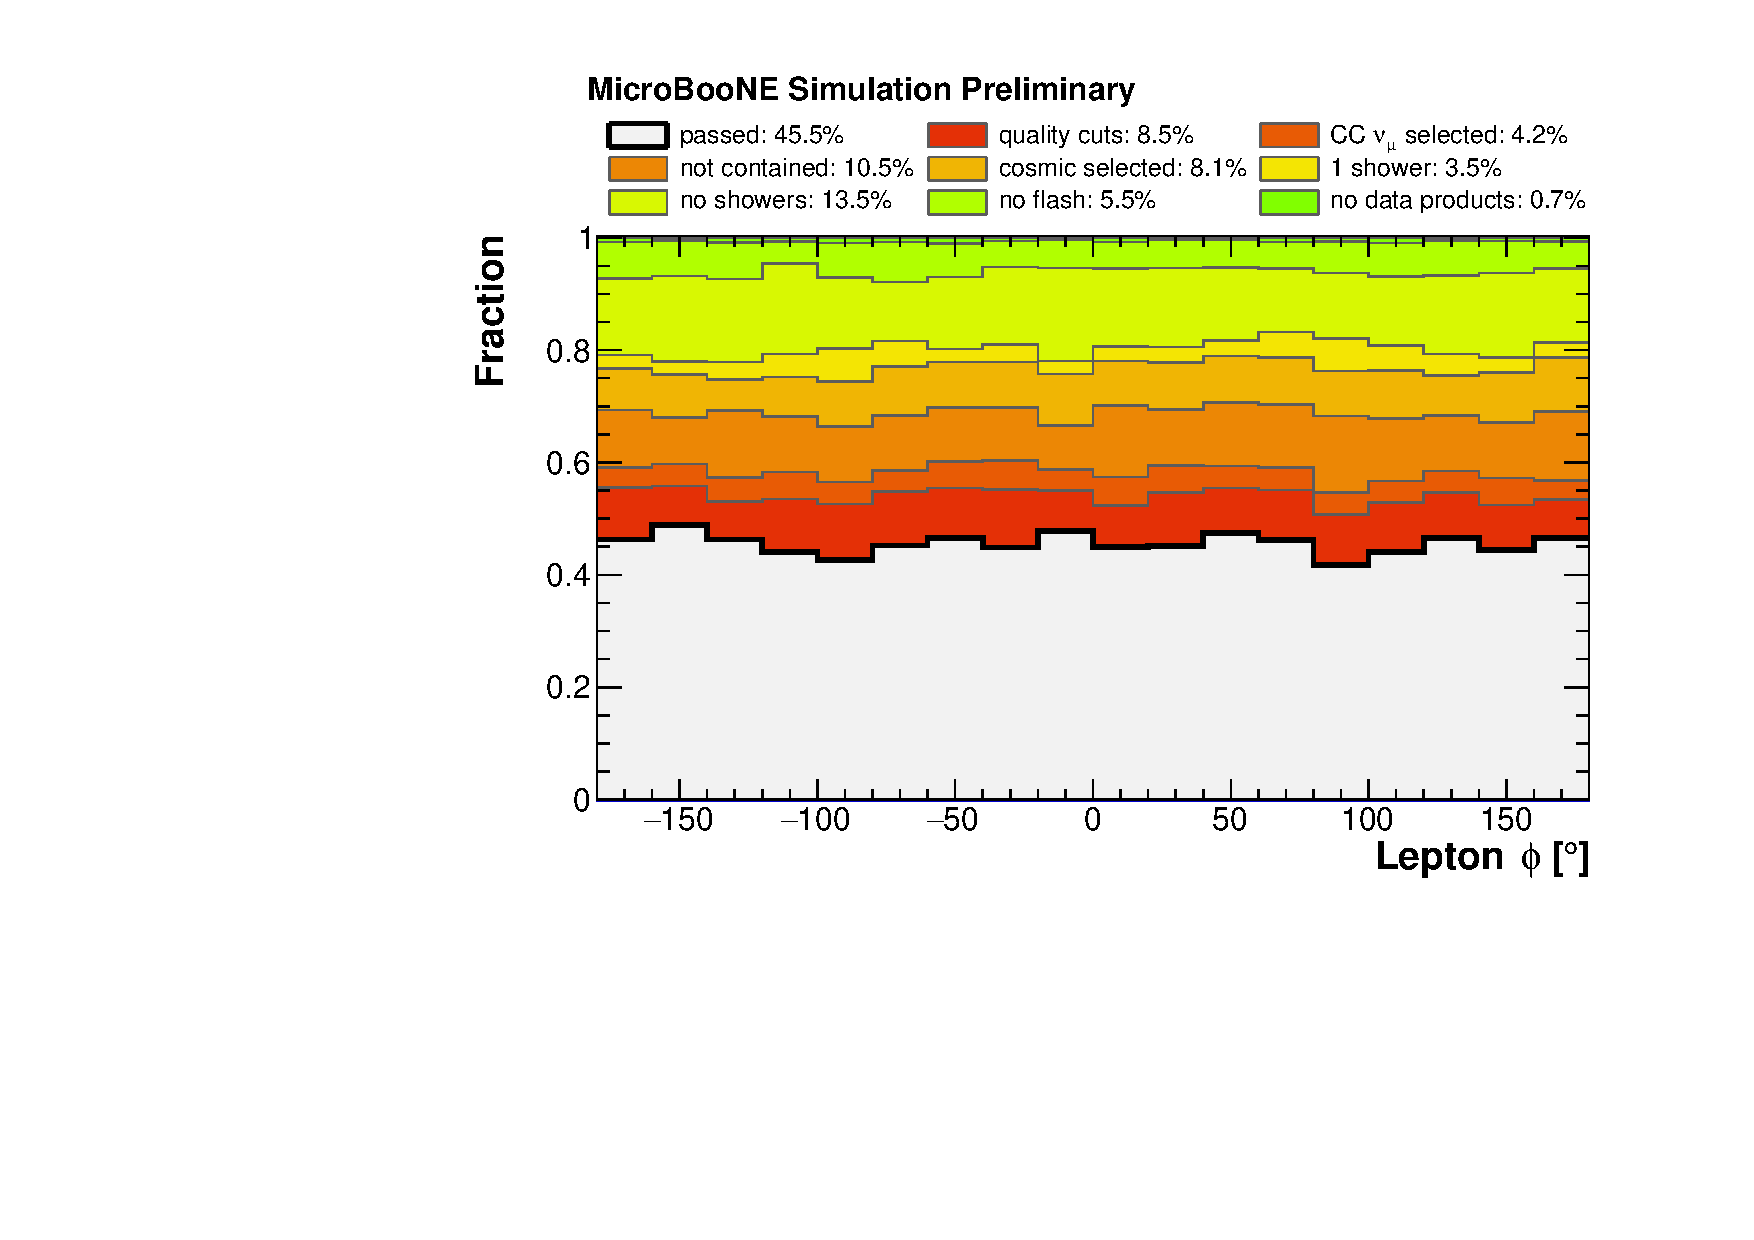
\includegraphics[width=\linewidth]{figures/ineff_phi.pdf}
    \caption{$\phi$ efficiency.} 
  \end{subfigure}
  \caption{Stacked histogram of generated events as a function of the electron $\theta$ (left) and $\phi$ (right) angles, categorised into correctly identified signal events {(\emph{passed})} and different reconstruction or identification failure modes.}
  \label{fig:ineff_angles}
\end{figure}

\subsection{Selection results}\label{sec:numu}
The previous selection efficiency results were performed with the $\nu_{e}$ CC0$\pi$-Np + cosmic sample. We now look at the selection performances when analysing events coming from the complete set of the events acquired by MicroBooNE, including non-$\nu_{e}$ events. In the \emph{BNB+cosmic} sample every event will have at least one neutrino interacting in the cryostat volume and triggering the detector, plus all the cosmic rays hitting the detector in the same readout window. In the data, however, this is not always true, since the detector can be triggered also by a cosmic ray producing a flash in the optical system during the beam window, without necessarily having a neutrino interaction. In order to estimate this background component, defined as \emph{in-time cosmic rays}, we have used the data sample collected with the \emph{data EXT} trigger.
The background caused by the neutrino interactions happening outside the cryostat has been evaluated using the \emph{dirt} sample.
We divide the selected events (signal and background) into 8 categories:
\begin{description}
\item[Beam intrinsic $\nu_{e}$ CC$0\pi$-Np:] charged-current $\nu_{e}$ neutrino interaction, at least one proton (N > 1), one electron, and no other visible particles above detection threshold. This category represents the signal of our analysis.
\item[Beam intrinsic $\nu_{e}$ CC:] charged-current $\nu_{e}$ neutrino interaction that is not $\nu_{e}$ CC$0\pi$-Np or where the electron or protons were below the detection threshold defined above.
\item[Beam intrinsic $\nu_{\mu}$:] charged-current $\nu_{\mu}$ neutrino interaction.
\item[Beam intrinsic NC:] neutral current neutrino interaction (both $\nu_{\mu}$ and $\nu_{e}$).
\item[Outside fiducial volume:] neutrino interaction which occurs outside the fiducial volume, but with one or more final-state particles inside in the fiducial volume.
\item[Cosmic contaminated:] neutrino interaction candidate with at least a cosmogenic track or shower, attached to a correctly reconstructed neutrino candidate.
\item[Cosmic:] there is a neutrino interaction in the event, but we select a cosmic-ray interaction happening during the same readout window as the neutrino candidate.
\item[Data off-beam]: event with no neutrino interaction, but where a cosmic-ray interaction in time-coincidence with the beam-gate window triggered the event, and activity was selected as a neutrino candidate.
\end{description}

Table \ref{tab:result} shows a summary of the selection algorithm results, with the corresponding number of events for each category.
%The numbers correspond to an exposure of the MicroBooNE detector of \num{4.34e19} protons on target (POT). This is equivalent to the amount of data analyzed here, which is a subset of the data collected from February to April 2016.

\begin{table}[htbp]
   \centering
      \caption{Summary of the selection results, showing the contribution of each event category, for a MicroBooNE exposure of \num{4.34e19} POT. Uncertainties are statistical only. {For the \emph{Cosmic contaminated} category the number of generated events correspond to the number of neutrino interactions inside the cryostat. For the \emph{Cosmic} category, it corresponds to the total number of simulated neutrino interactions, both inside and outside the cryostat.}}\label{tab:result}
   \begin{tabular}{llrrrrr}
     \toprule
     Category & Generated & Selected & Efficiency \\
     \midrule

     \textbf{$\nu_{e}$ CC0$\pi$-Np (signal)}  & $33.8$    & $15.4$  & $(45.5\pm0.5)$~\%\\
     $\nu_{e}$ CC                             & $39.5$    & $15.4$  & $(39.0\pm0.5)$~\%\\
     Beam intrinsic $\nu_{\mu}$               & $10905.9$ & $488.9$ & $(4.5\pm0.2)$~\%\\
     Beam intrinsic NC                        & $3532.8$  & $329.5$ & $(9.3\pm0.2)$~\%\\
     Outside fid. vol.                        & $36634.6$ & $79.0$  & $(0.2\pm0.1)$~\%\\
     Data off-beam                            & $123070.2$ & $1593.4$ & $(1.3\pm0.1)$~\%\\
     Cosmic contaminated                      & $14706.4$  & $376.1$  & $(2.5\pm0.1)$~\%\\ 
     Cosmic                                   & $51356.1$  & $489.4$  & $(0.8\pm0.1)$~\%\\

     \bottomrule
   \end{tabular}

\end{table}

Each selected event has a neutrino interaction candidate with one or more tracks and one or more showers associated with the interaction vertex. Since we use two different methods to measure the energy of the tracks and the energy of the showers (see Section \ref{sec:energyreco}), it is necessary to verify the agreement between the shower multiplicity and track multiplicity distributions in data and Monte Carlo. Figure \ref{fig:multiplicity} shows that the two distributions agree within the systematic uncertainties, whose evaluation is described in Section \ref{sec:systematics}.

\begin{figure}[htbp]
\centering
  \begin{subfigure}{0.49\textwidth}
    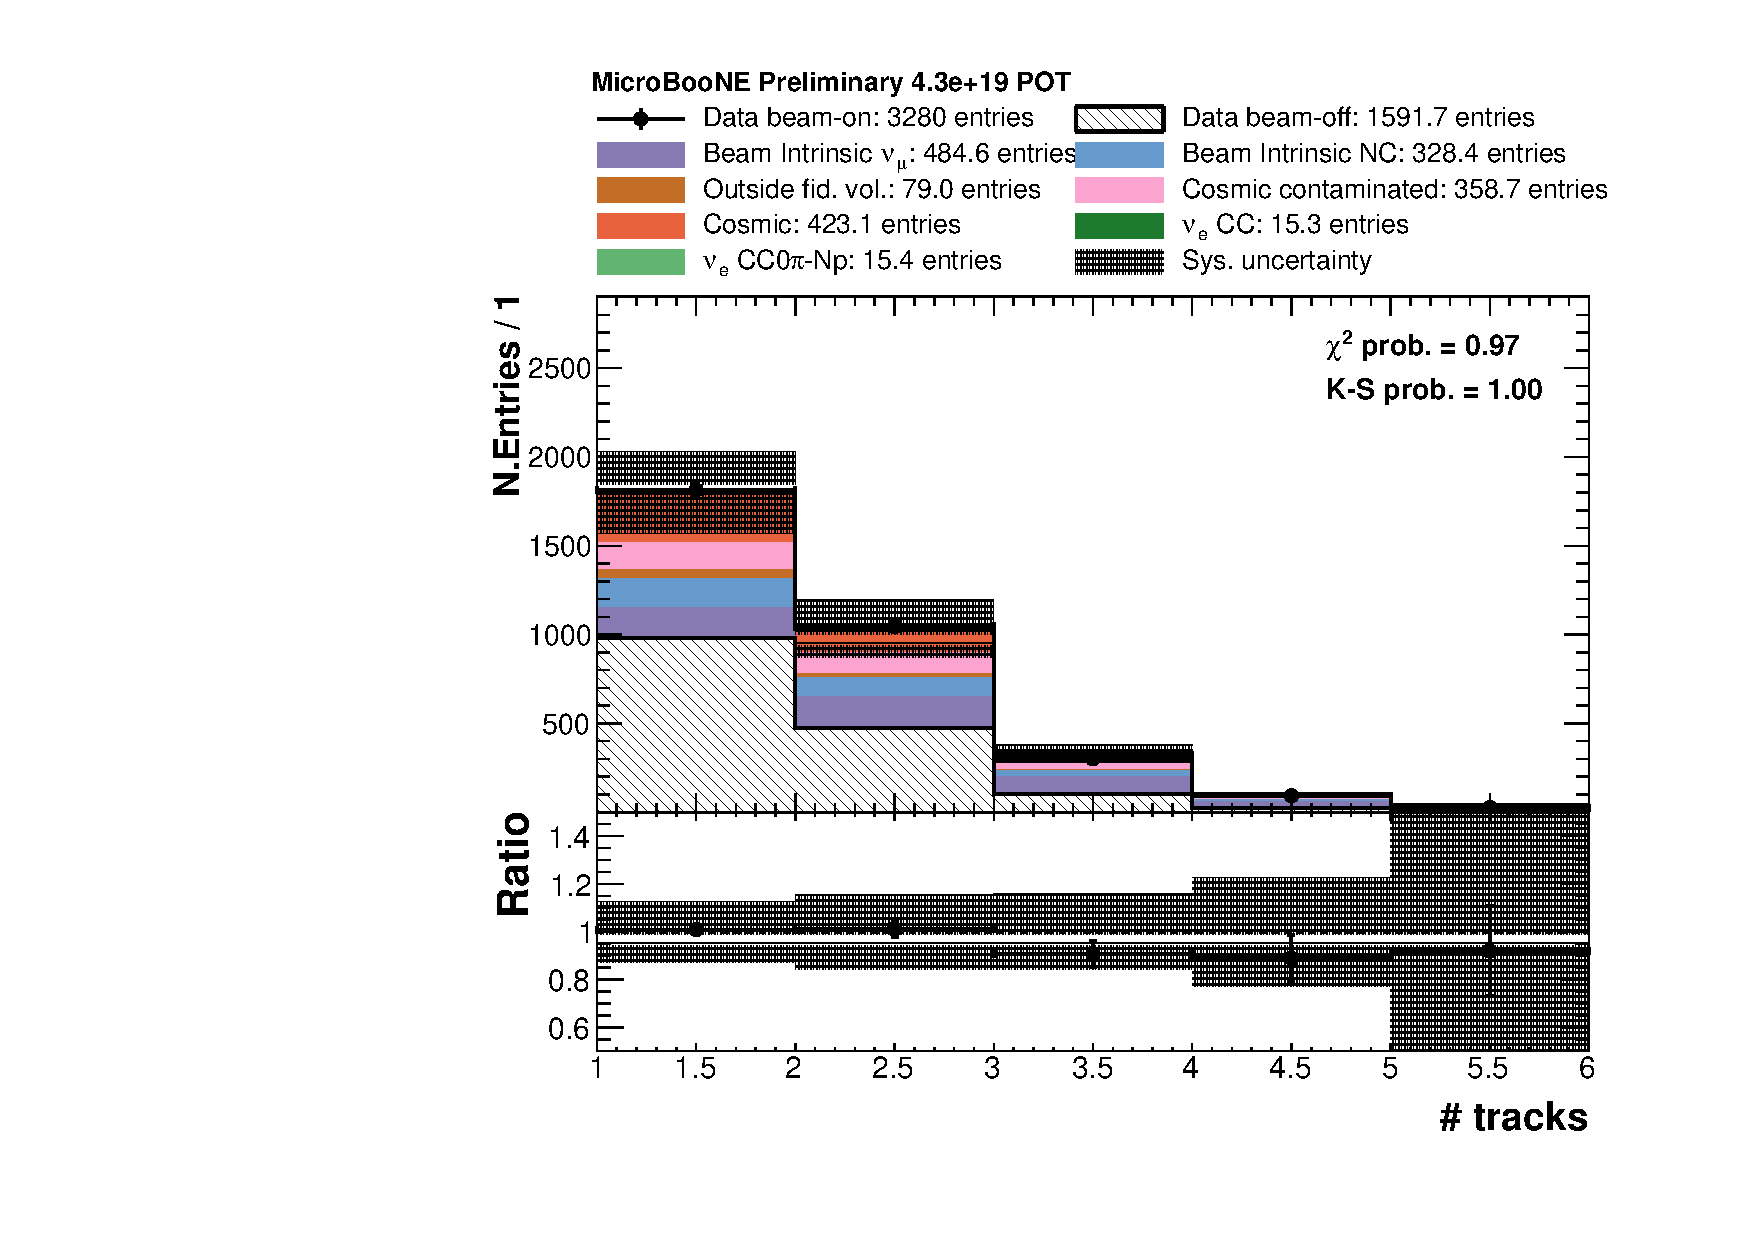
\includegraphics[width=\linewidth]{figures/n_tracks.pdf}
    \caption{Track multiplicity.} 
  \end{subfigure}\hfill
    \begin{subfigure}{0.49\textwidth}
    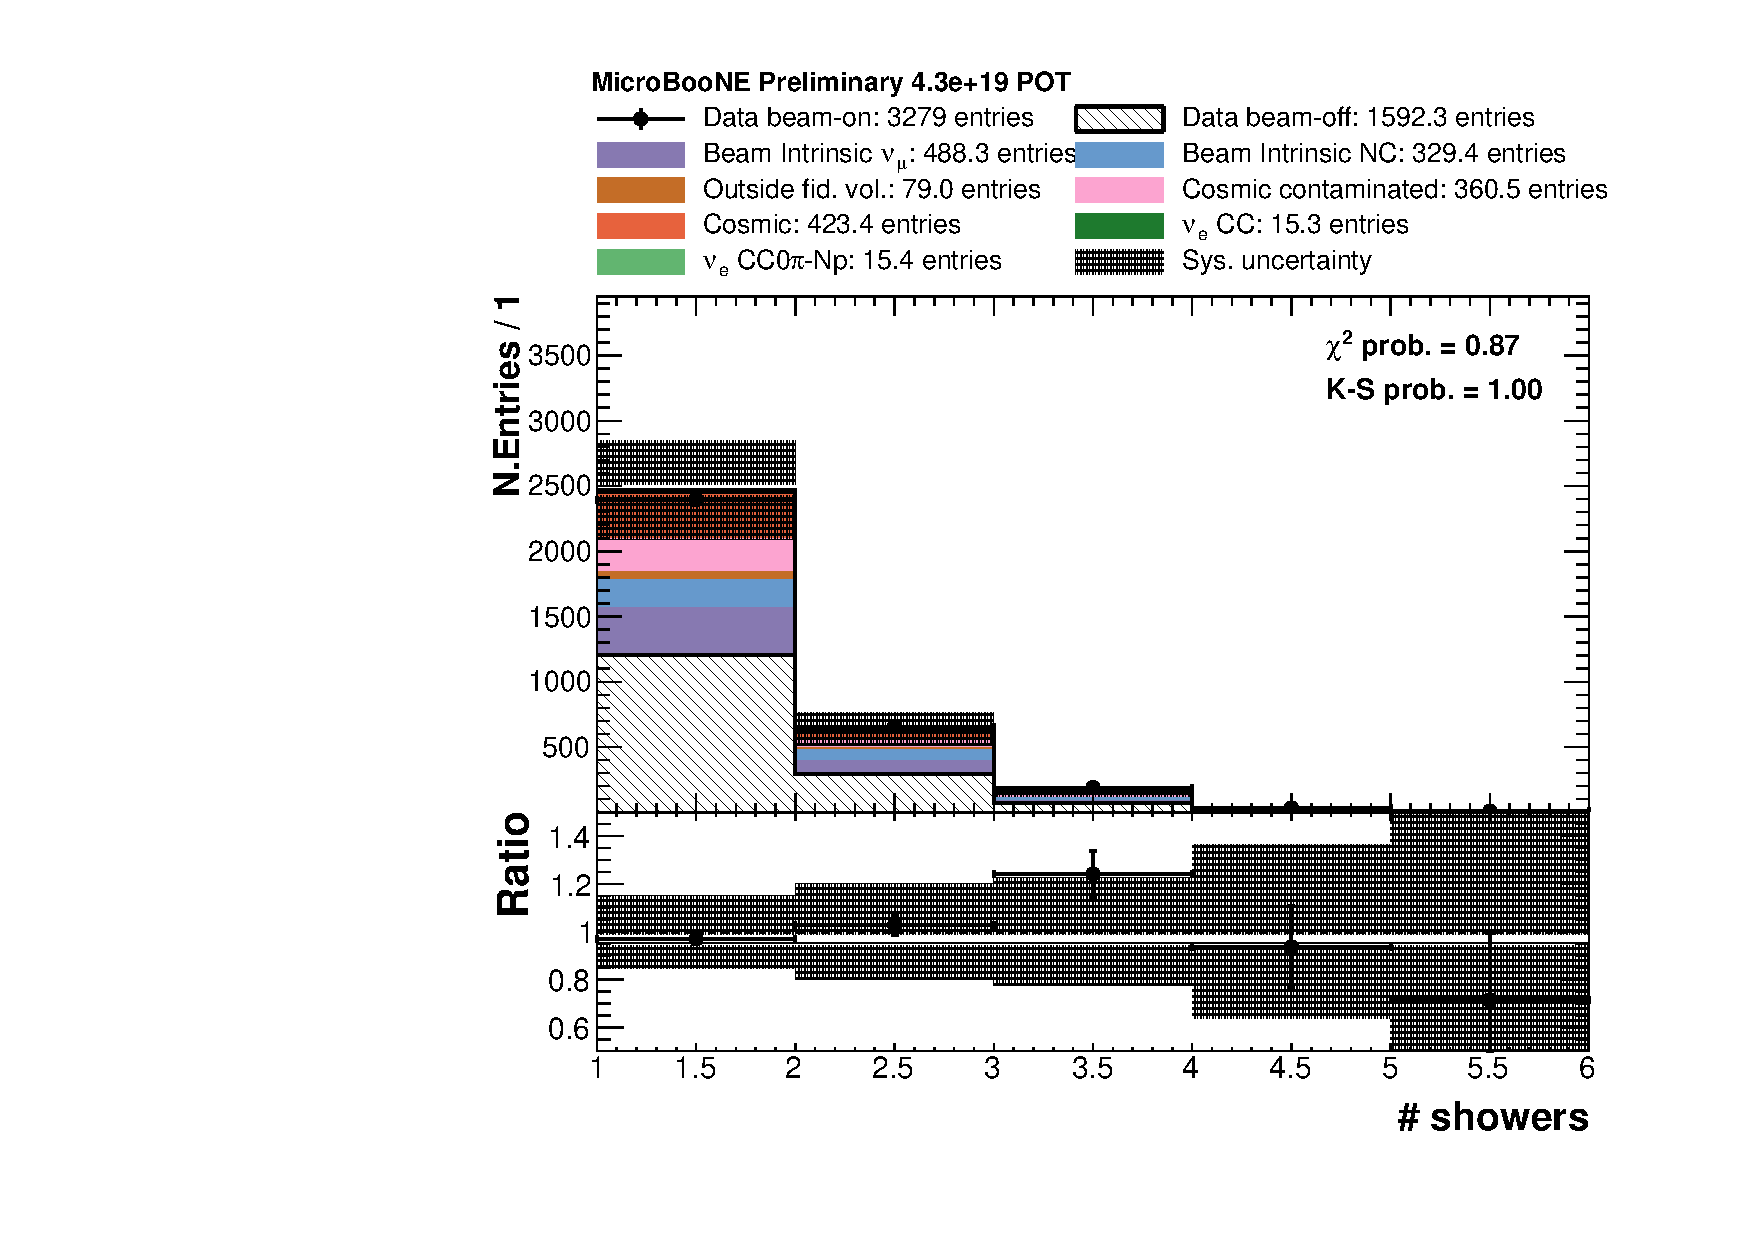
\includegraphics[width=\linewidth]{figures/n_showers.pdf}
    \caption{Shower multiplicity.} 
  \end{subfigure}
  \caption{Distributions of the track and shower multiplicities in data and Monte Carlo simulation.}\label{fig:multiplicity}
\end{figure}

Figure \ref{fig:spectrum} shows the reconstructed deposited energy spectrum of the selected events. The reconstructed deposited energy $E_{\mathrm{deposited}}$ has been measured with the procedure described in Section \ref{sec:depositedenergy}. Both the $\chi^2$ and Kolmogorov-Smirnov tests give a probability of 1.00 (rounded up at the second decimal digit) of the null hypothesis, which is the data distribution being compatible with the Monte Carlo simulation.
%This plot shows that our selection procedure has similar performances in data and Monte Carlo and that there is no evident bias in the energy reconstruction. 

\begin{figure}[htbp]
\centering
  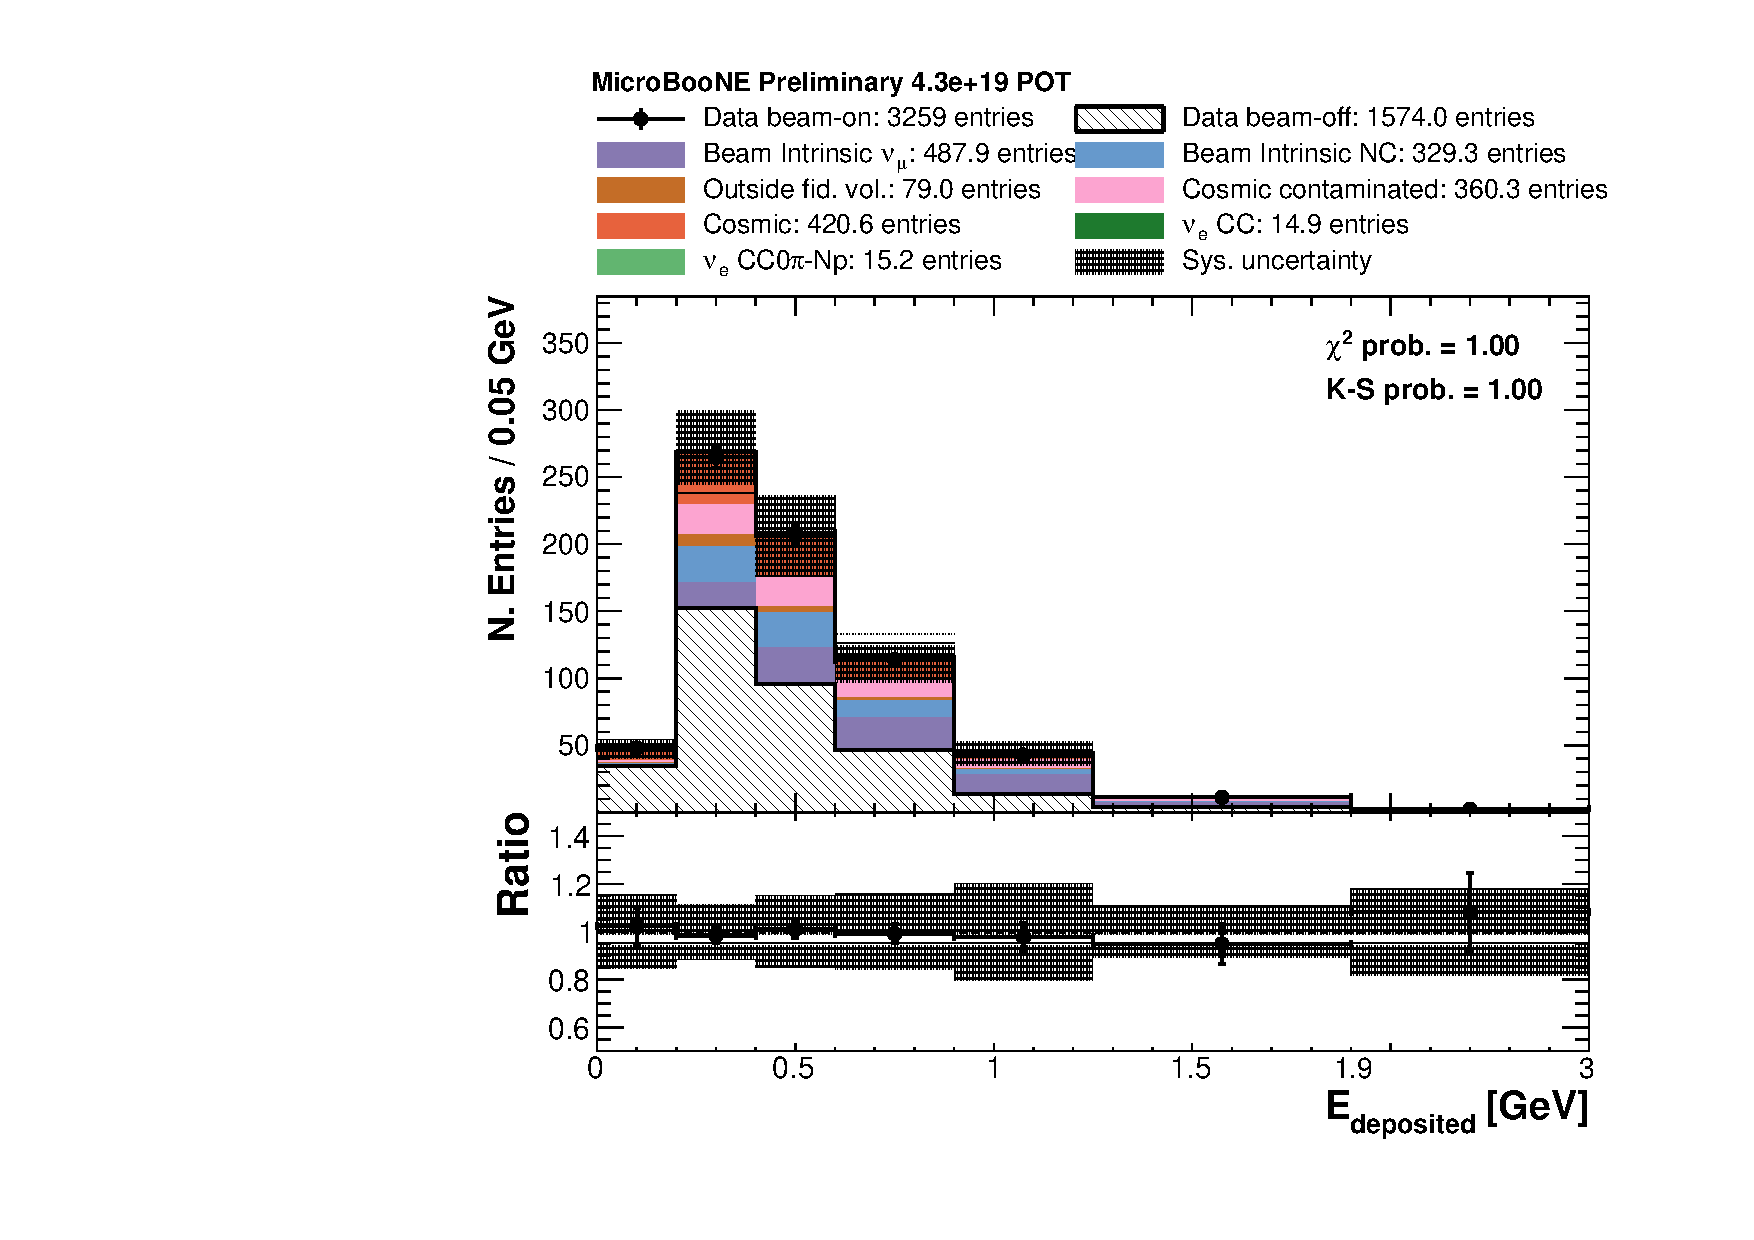
\includegraphics[width=0.65\linewidth]{figures/h_fixed_energy.pdf}
  \caption{Reconstructed energy spectrum after the event selection algorithm and the veto of the events selected by the CC $\nu_{\mu}$ module. The histograms of the event categories are stacked.}
  \label{fig:spectrum}
\end{figure}

The agreement between data and simulation is also verified in the angular distributions of the reconstructed showers objects, shown in Figure \ref{fig:thetaphi}. As expected, the neutrino distributions are mostly constant as a function of the azimuthal angle $\phi$ and peaked at low inclination angle $\theta$ values, since the interactions are mostly forward going. The inclination angle $\theta$ distribution agrees within the uncertainties both for shape and normalisation. The azimuthal angle $\phi$ distribution shows a slight disagreement around $\phi = 0^{\circ}$ and $\phi = \pm180^{\circ}$. This is caused by an imprecise signal simulation that predominantly affects tracks moving exactly towards or away from the anode \cite{Adams:2018gbi}. This effect is taken into account in the Dynamic Induced Charge detector systematic sample (Section \ref{sec:systematics}). 

Figure \ref{fig:thetaphi_pdg} shows the angular distributions classified according to the primary particle that generated the shower (in the case of a Michel electron the shower is placed in the muon category). Each entry in the histogram correspond to a reconstructed shower, so it is possible to have more than one entry per event. As expected, the $\theta$ distribution is peaked at low angles, since neutrino interactions are mostly forward-going. The $\phi$ distribution is mainly flat for neutrino-induced particles (electrons, photons) and with two peaks at $\pm90^{\circ}$ for mostly-vertical cosmic-induced particles (mainly muons). In this case, the data points correspond to the bin-by-bin statistical subtraction of the beam-on and beam-off entries.

\begin{figure}[htbp]
\centering
  \begin{subfigure}{0.49\textwidth}
    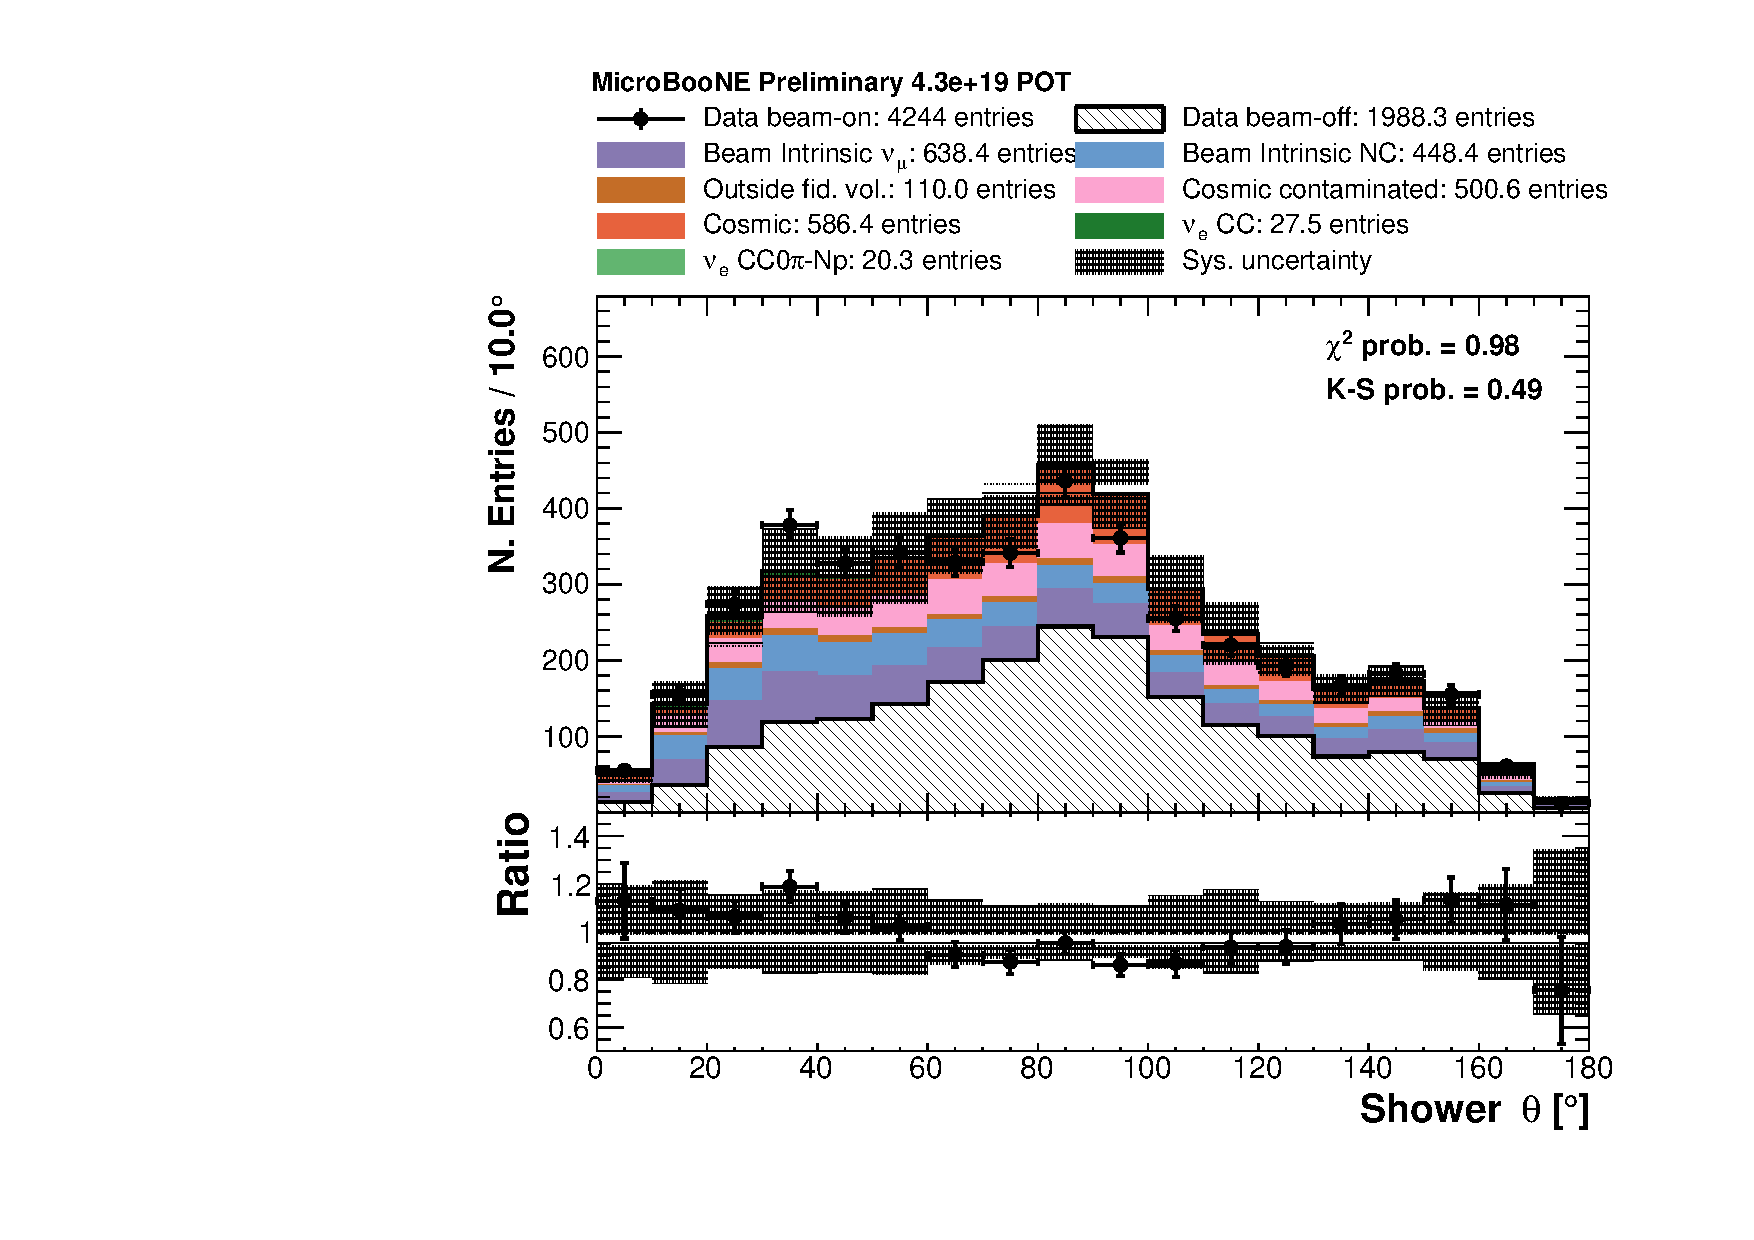
\includegraphics[width=\linewidth]{figures/h_shower_theta.pdf}
    \caption{Inclination angle $\theta$.} 
  \end{subfigure}\hfill
    \begin{subfigure}{0.49\textwidth}
    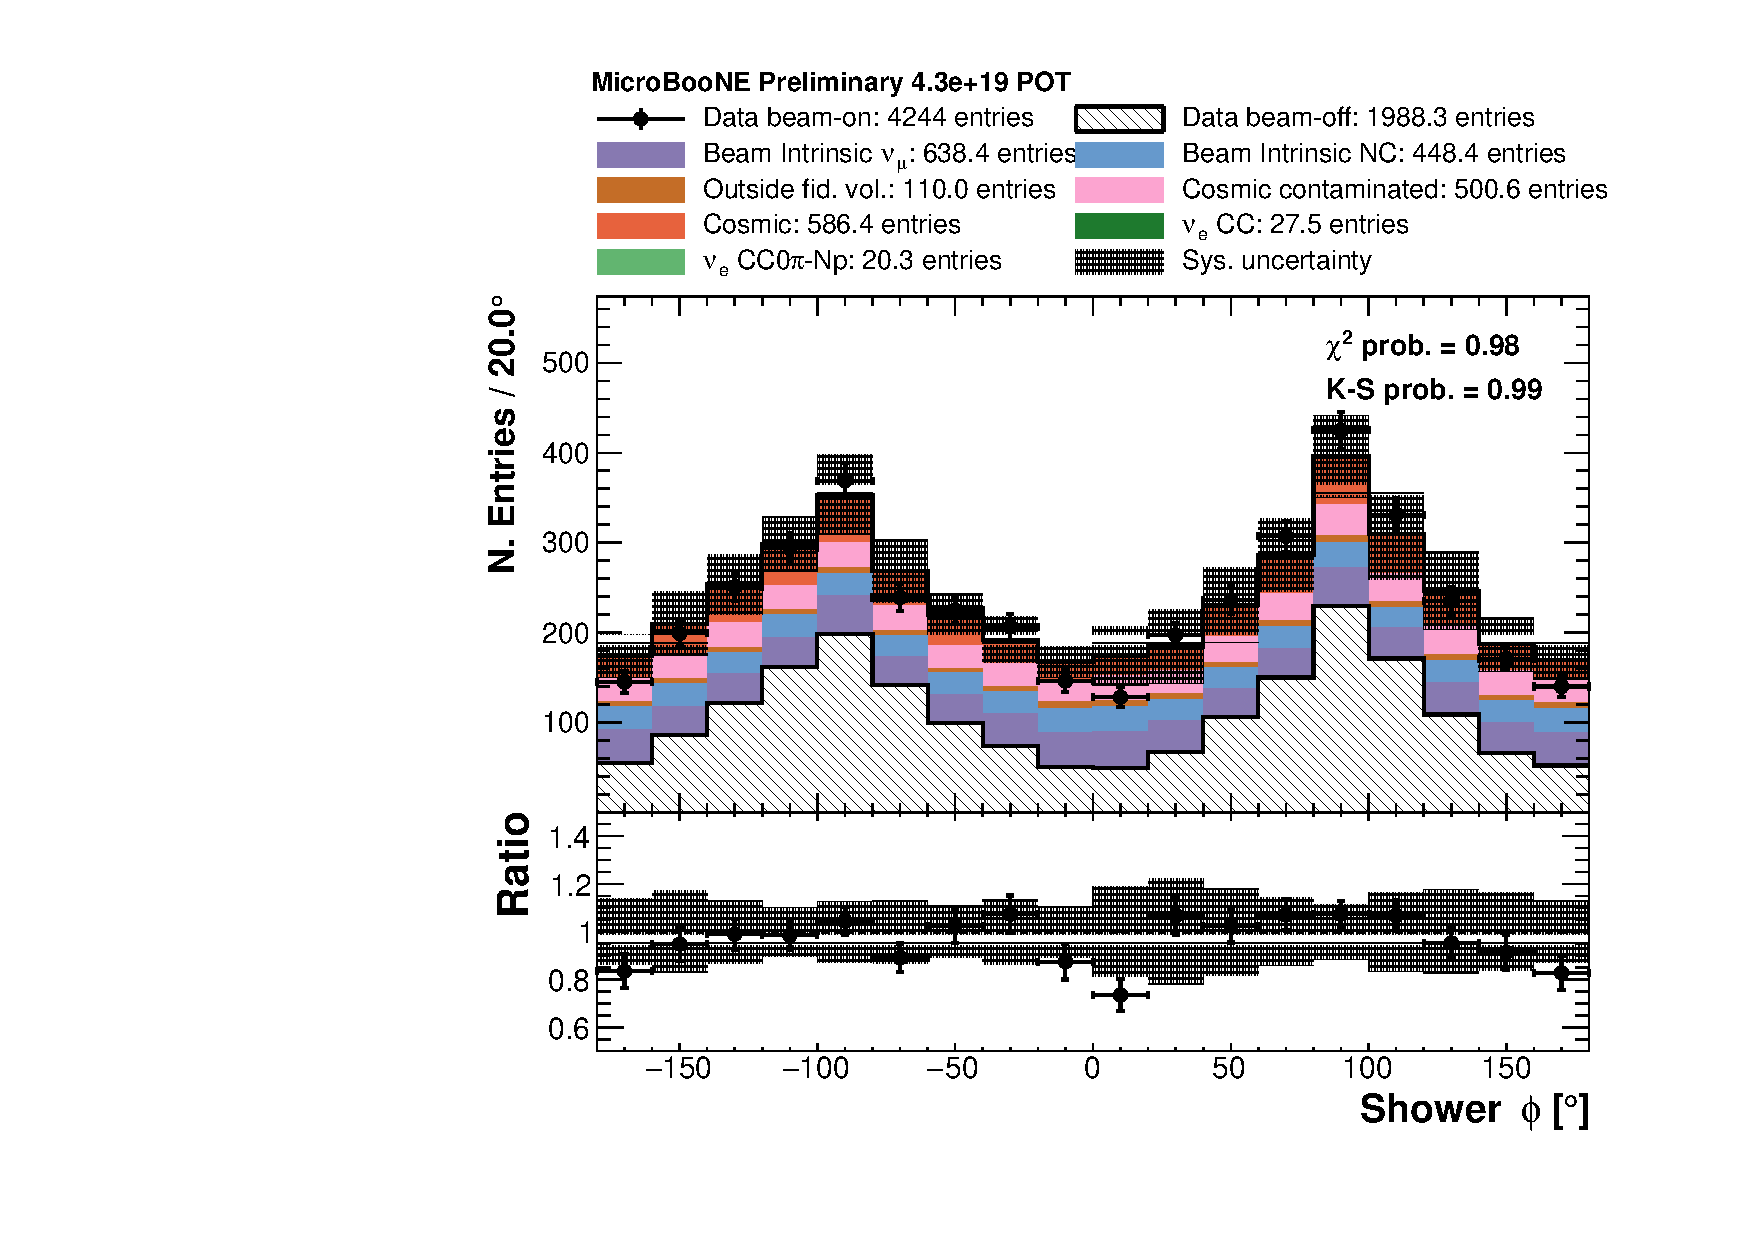
\includegraphics[width=\linewidth]{figures/h_shower_phi.pdf}
    \caption{Azimuthal angle $\phi$.} 
  \end{subfigure}
  \caption{Distributions of the inclination angle $\theta$ and the azimuthal angle $\phi$ of the reconstructed showers in the selected events for each event category.}\label{fig:thetaphi}
\end{figure}

\begin{figure}[htbp]
\centering
  \begin{subfigure}{0.49\textwidth}
    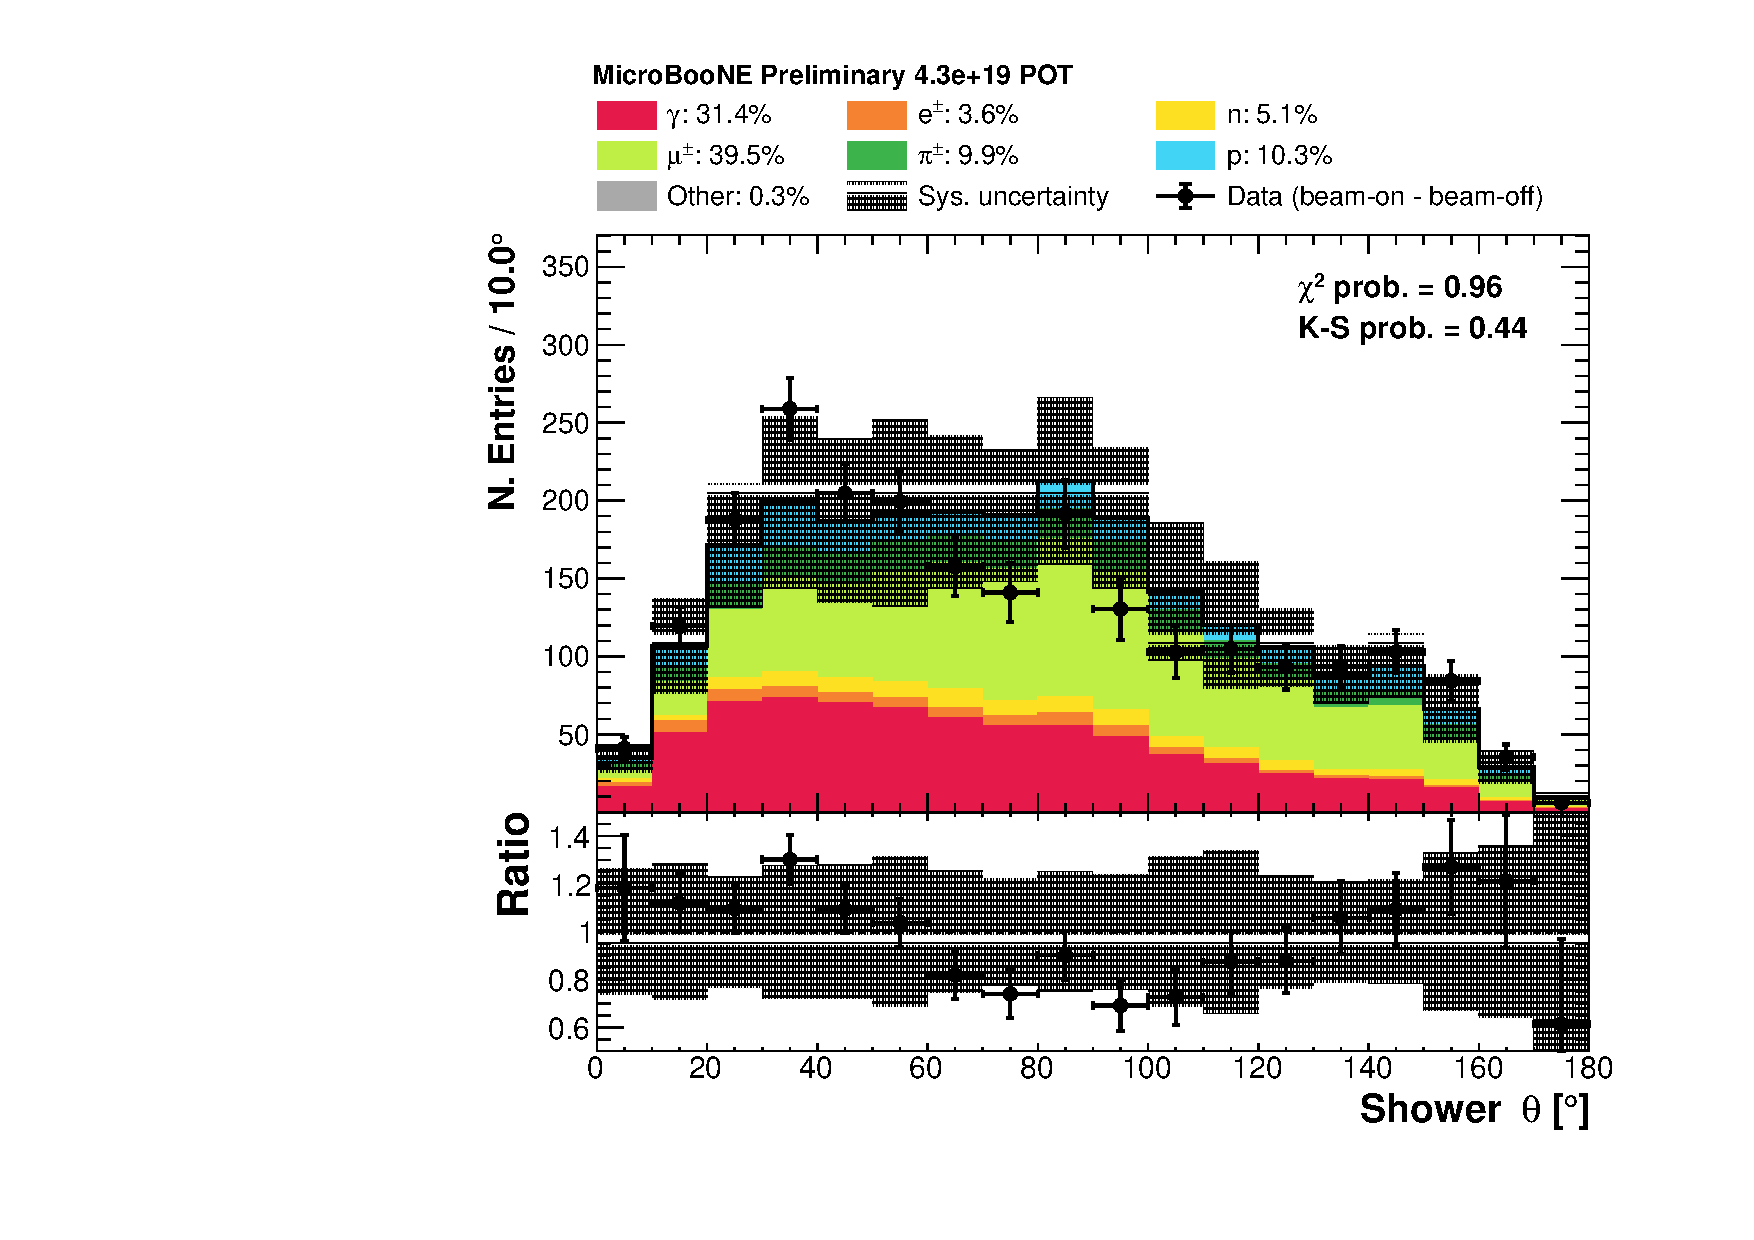
\includegraphics[width=\linewidth]{figures/h_shower_theta_pdg.pdf}
    \caption{Inclination angle $\theta$.} 
  \end{subfigure}
    \begin{subfigure}{0.49\textwidth}
    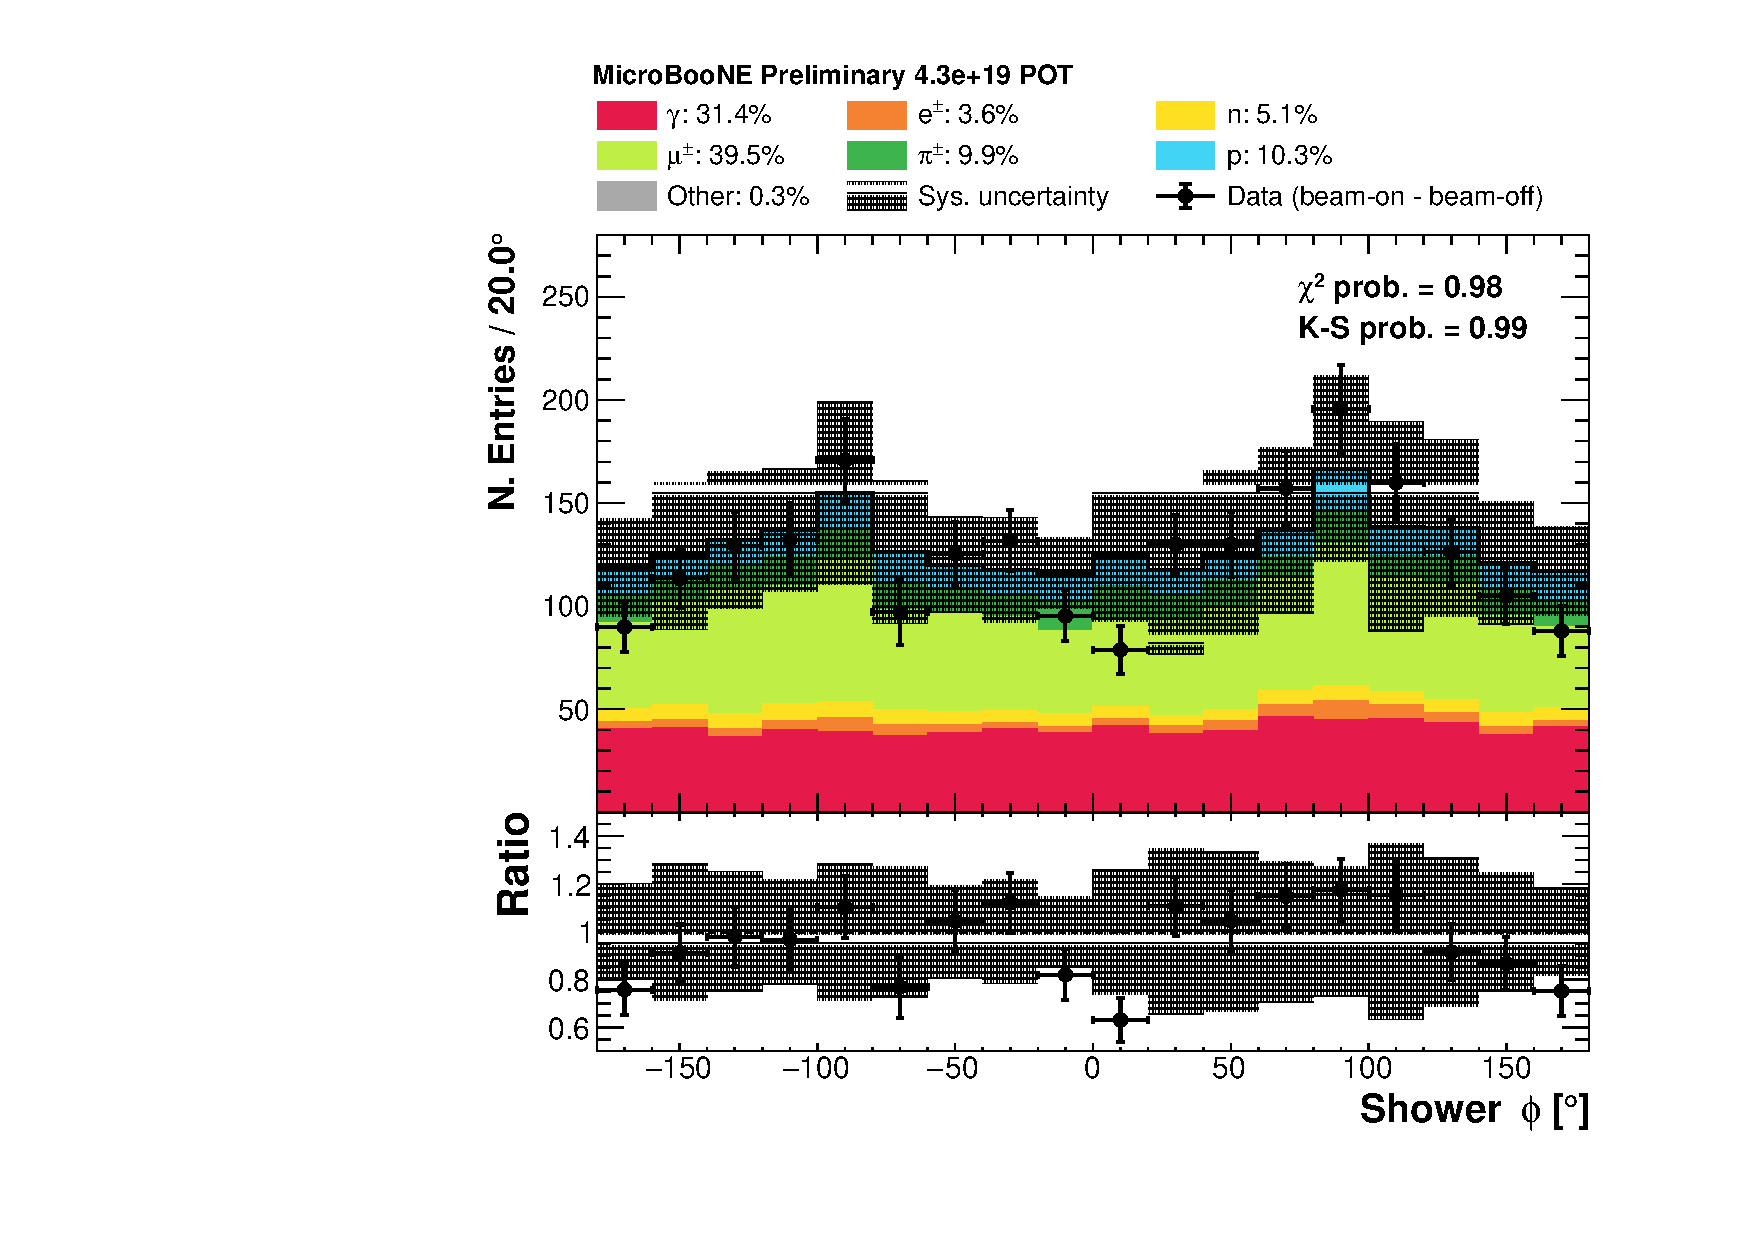
\includegraphics[width=\linewidth]{figures/h_shower_phi_pdg.pdf}
    \caption{Azimuthal angle $\phi$.} 
  \end{subfigure}
  \caption{{Distributions of the inclination angle $\theta$ and the azimuthal angle $\phi$ of the reconstructed showers, classified according to the primary particle that generated them.}}\label{fig:thetaphi_pdg}
\end{figure}

A small fraction of the data events was also visually inspected: Figure \ref{fig:evds} shows three event displays of data events compatible with a $\nu_{e}$ CC0$\pi$-Np interaction. 

\begin{figure}[htbp]
\centering
  \begin{subfigure}{0.45\textwidth}
  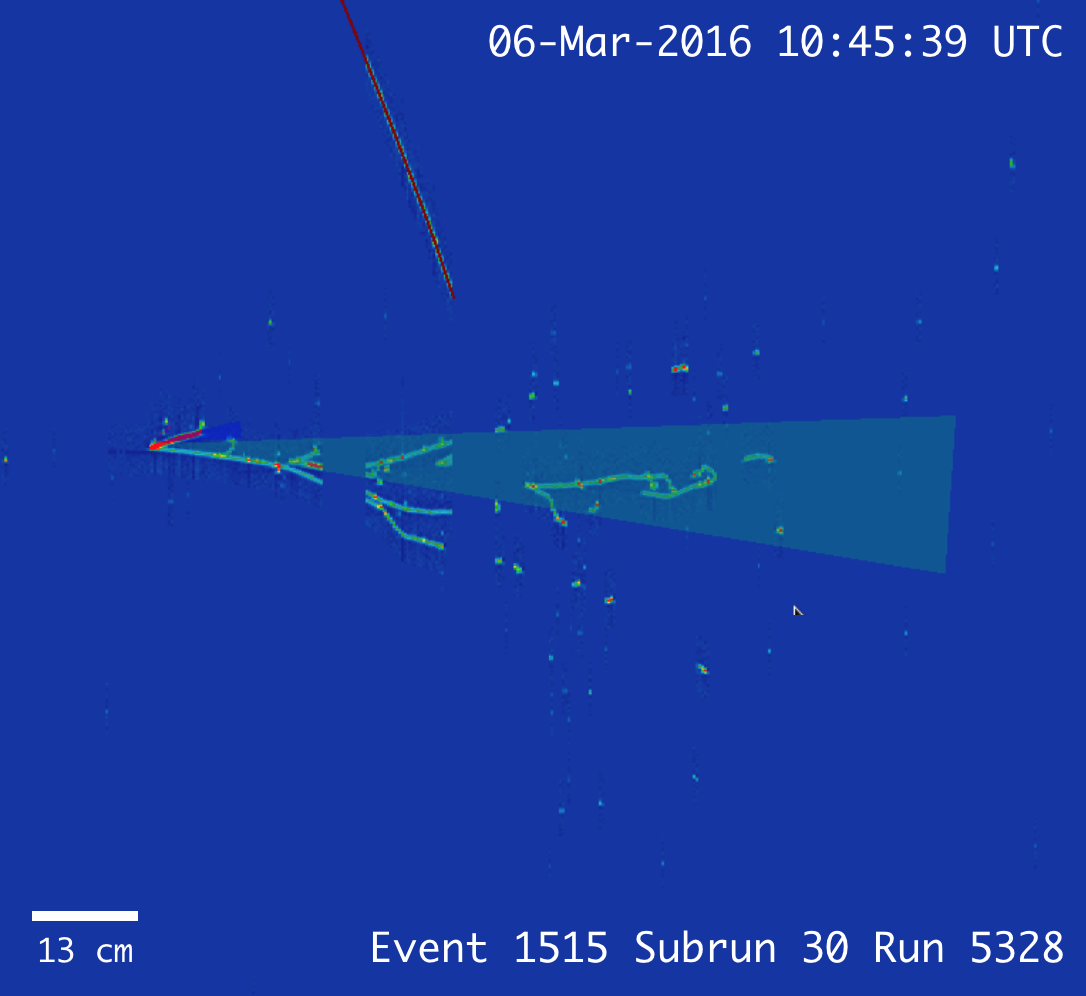
\includegraphics[width=\linewidth]{figures/data3.png}
    \caption{Event 1515, Subrun 30, Run 5328}\end{subfigure}
  \hfill\begin{subfigure}{0.45\textwidth}	
  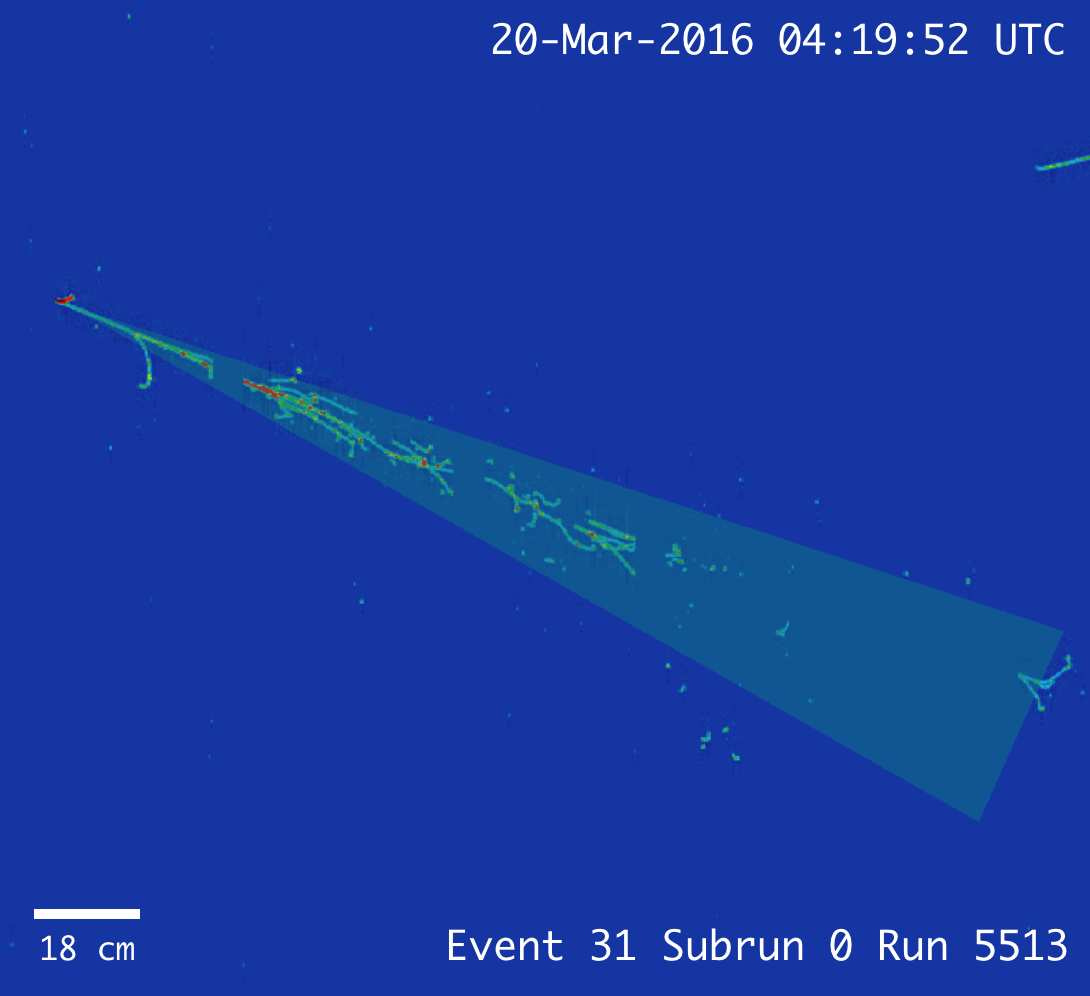
\includegraphics[width=\linewidth]{figures/data2.png}
  \caption{Event 31, Subrun 0, Run 5513}
\end{subfigure}
\vspace{1em}

  \begin{subfigure}{0.45\textwidth}	
  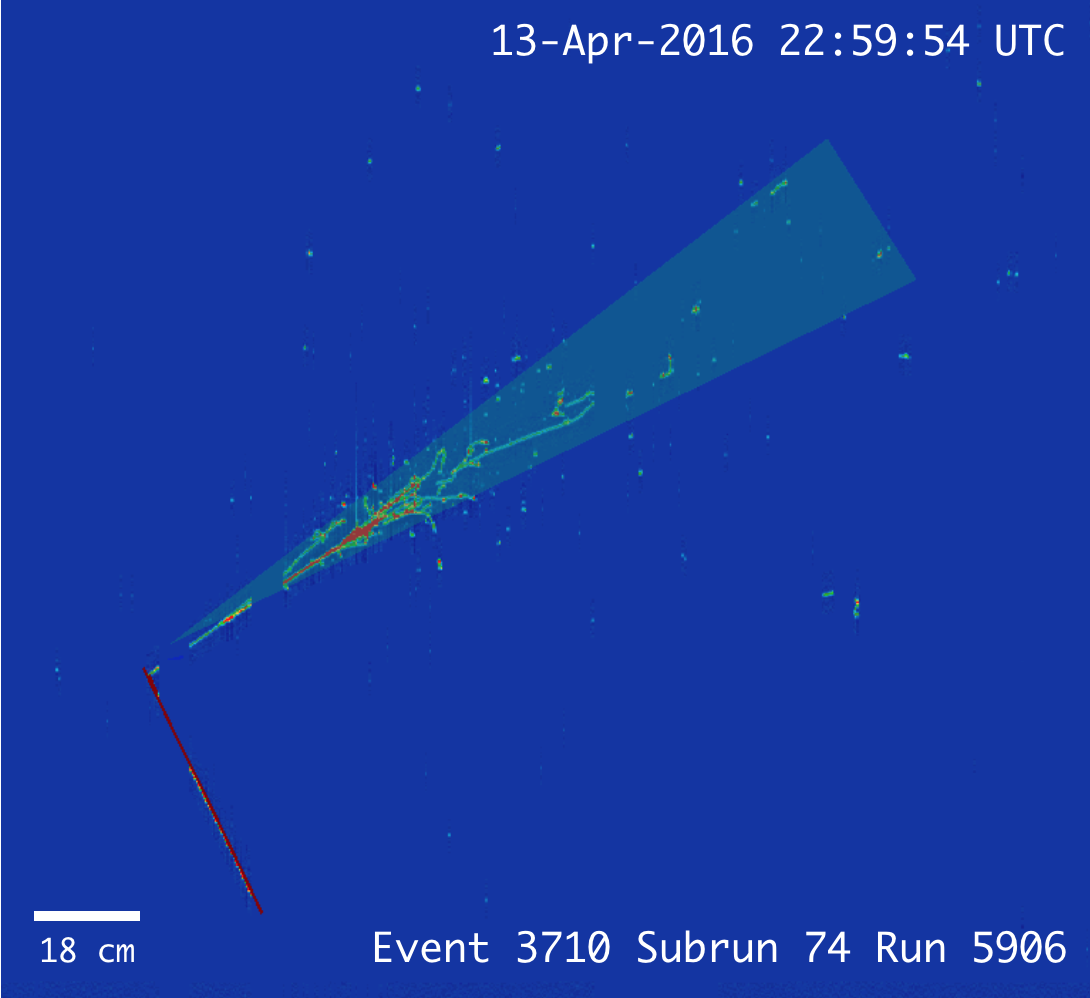
\includegraphics[width=\linewidth]{figures/data1.png}
  \caption{Event 3710, Subrun 74, Run 5906}
\end{subfigure}

  \caption{Event displays of the collection plane of three $\nu_{e}$-like data events selected by our algorithm. The gaps are caused by the presence of missing or unresponsive wires. The red lines correspond to reconstructed track-like objects and the green cones correspond to reconstructed shower-like objects. }
  \label{fig:evds}
\end{figure}
